\documentclass[11pt,a4paper]{report}

% ============================================================================
% PACKAGES
% ============================================================================
\usepackage[utf8]{inputenc}
\usepackage[T1]{fontenc}
\usepackage[margin=1in, headheight=14pt]{geometry}
\usepackage{graphicx}
\usepackage{xcolor}
\usepackage{titlesec}
\usepackage{titletoc}
\usepackage{fancyhdr}
\usepackage{enumitem}
\usepackage{booktabs}
\usepackage{longtable}
\usepackage{tabularx}
\usepackage{multirow}
\usepackage{hyperref}
\usepackage{tcolorbox}
\usepackage{tikz}
\usepackage{pgfplots}
\usepackage{array}
\usepackage{colortbl}
\usepackage{pifont}
\usepackage{parskip}
\usepackage{caption}
\usepackage{float}
\usepackage{calc}
\usepackage{calc}
\usepackage{amsmath}
\usepackage{amssymb}


\pgfplotsset{compat=1.18}
\usetikzlibrary{shapes.geometric, arrows, positioning, calc, decorations.pathreplacing, backgrounds, fit, matrix}

% ============================================================================
% COLOR DEFINITIONS
% ============================================================================
\definecolor{primaryblue}{RGB}{0, 82, 147}
\definecolor{secondaryblue}{RGB}{0, 120, 190}
\definecolor{accentorange}{RGB}{255, 140, 0}
\definecolor{lightgray}{RGB}{245, 245, 245}
\definecolor{darkgray}{RGB}{64, 64, 64}
\definecolor{successgreen}{RGB}{40, 167, 69}
\definecolor{warningyellow}{RGB}{255, 193, 7}
\definecolor{dangerred}{RGB}{220, 53, 69}
\definecolor{purpleaccent}{RGB}{111, 66, 193}
\definecolor{tealaccent}{RGB}{32, 156, 157}

% Maturity level colors
\definecolor{crawlcolor}{RGB}{255, 99, 71}
\definecolor{walkcolor}{RGB}{255, 193, 7}
\definecolor{runcolor}{RGB}{40, 167, 69}

% ============================================================================
% TCOLORBOX DEFINITIONS
% ============================================================================
\tcbuselibrary{skins,breakable}

\newtcolorbox{objectivebox}{
    colback=primaryblue!5,
    colframe=primaryblue,
    fonttitle=\bfseries,
    title=Strategic Objectives,
    breakable,
    left=5pt,
    right=5pt,
    top=5pt,
    bottom=5pt
}

\newtcolorbox{keyconceptbox}{
    colback=accentorange!10,
    colframe=accentorange,
    fonttitle=\bfseries,
    title=Key Concept,
    breakable,
    left=5pt,
    right=5pt
}

\newtcolorbox{successbox}{
    colback=successgreen!5,
    colframe=successgreen,
    fonttitle=\bfseries,
    title=Success Criteria,
    breakable,
    left=5pt,
    right=5pt
}

\newtcolorbox{actionbox}{
    colback=secondaryblue!5,
    colframe=secondaryblue,
    fonttitle=\bfseries,
    title=Action Items,
    breakable,
    left=5pt,
    right=5pt
}

\newtcolorbox{notebox}{
    colback=lightgray,
    colframe=darkgray,
    fonttitle=\bfseries,
    title=Important Note,
    breakable,
    left=5pt,
    right=5pt
}

\newtcolorbox{warningbox}{
    colback=warningyellow!10,
    colframe=warningyellow!80!black,
    fonttitle=\bfseries,
    title=Risk Consideration,
    breakable,
    left=5pt,
    right=5pt
}

\newtcolorbox{milestonebox}{
    colback=purpleaccent!5,
    colframe=purpleaccent,
    fonttitle=\bfseries,
    breakable,
    left=5pt,
    right=5pt
}

\newtcolorbox{deliverablebox}{
    colback=tealaccent!5,
    colframe=tealaccent,
    fonttitle=\bfseries,
    title=Key Deliverables,
    breakable,
    left=5pt,
    right=5pt
}

\newtcolorbox{phasebox}[1][]{
    colback=primaryblue!3,
    colframe=primaryblue,
    fonttitle=\bfseries,
    breakable,
    left=8pt,
    right=8pt,
    top=8pt,
    bottom=8pt,
    #1
}

% ============================================================================
% TITLE FORMATTING
% ============================================================================
\titleformat{\chapter}[display]
{\normalfont\huge\bfseries\color{primaryblue}}
{\chaptertitlename\ \thechapter}{20pt}{\Huge}

\titleformat{\section}
{\normalfont\Large\bfseries\color{secondaryblue}}
{\thesection}{1em}{}

\titleformat{\subsection}
{\normalfont\large\bfseries\color{darkgray}}
{\thesubsection}{1em}{}

\titleformat{\subsubsection}
{\normalfont\normalsize\bfseries\color{darkgray}}
{\thesubsubsection}{1em}{}

% ============================================================================
% HEADER/FOOTER
% ============================================================================
\pagestyle{fancy}
\fancyhf{}
\fancyhead[L]{\leftmark}
\fancyhead[R]{\textcolor{primaryblue}{Cloud FinOps Program Roadmap}}
\fancyfoot[C]{\thepage}
\renewcommand{\headrulewidth}{0.5pt}
\renewcommand{\footrulewidth}{0.3pt}

% ============================================================================
% HYPERREF SETUP
% ============================================================================
\hypersetup{
    colorlinks=true,
    linkcolor=primaryblue,
    urlcolor=secondaryblue,
    citecolor=darkgray,
    pdftitle={Cloud FinOps Program Roadmap},
    pdfauthor={Enterprise FinOps Initiative},
    pdfsubject={Comprehensive FinOps Implementation Roadmap}
}

% ============================================================================
% CUSTOM COMMANDS
% ============================================================================
% Preserve existing \checkmark (e.g., from amssymb) before redefining.
\let\amscheckmark\checkmark
\providecommand{\checkmark}{}
\renewcommand{\checkmark}{\textcolor{successgreen}{\ding{51}}}


\newcommand{\xmark}{\textcolor{dangerred}{\ding{55}}}
\newcommand{\duration}[1]{\textcolor{darkgray}{$\triangleright$ #1}}
\newcommand{\maturitylevel}[1]{%
    \ifnum#1=1\textcolor{crawlcolor}{\textbf{CRAWL}}%
    \else\ifnum#1=2\textcolor{walkcolor}{\textbf{WALK}}%
    \else\textcolor{runcolor}{\textbf{RUN}}%
    \fi\fi
}
\newcommand{\priority}[1]{%
    \ifnum#1=1\colorbox{dangerred!20}{\textcolor{dangerred}{\textbf{Critical}}}%
    \else\ifnum#1=2\colorbox{warningyellow!20}{\textcolor{warningyellow!80!black}{\textbf{High}}}%
    \else\colorbox{successgreen!20}{\textcolor{successgreen}{\textbf{Medium}}}%
    \fi\fi
}


% ============================================================================
% DOCUMENT BEGIN
% ============================================================================
\begin{document}

% ============================================================================
% TITLE PAGE
% ============================================================================
\begin{titlepage}
    \centering
    \vspace*{0.5cm}
    
    \begin{tikzpicture}[remember picture, overlay]
        \fill[primaryblue] (current page.north west) rectangle ([yshift=-5cm]current page.north east);
        \node[anchor=north, white, font=\Huge\bfseries] at ([yshift=-2cm]current page.north) {CLOUD FINOPS};
        \node[anchor=north, white, font=\Large] at ([yshift=-3.5cm]current page.north) {Program Implementation Roadmap};
    \end{tikzpicture}
    
    \vspace{5cm}
    
    {\Large\textcolor{darkgray}{A Comprehensive, Technology-Agnostic Guide for}\\[0.3cm]}
    {\Large\textcolor{darkgray}{Enterprise Cloud Financial Management Excellence}\\[2cm]}
    
    % Maturity Journey Visualization
    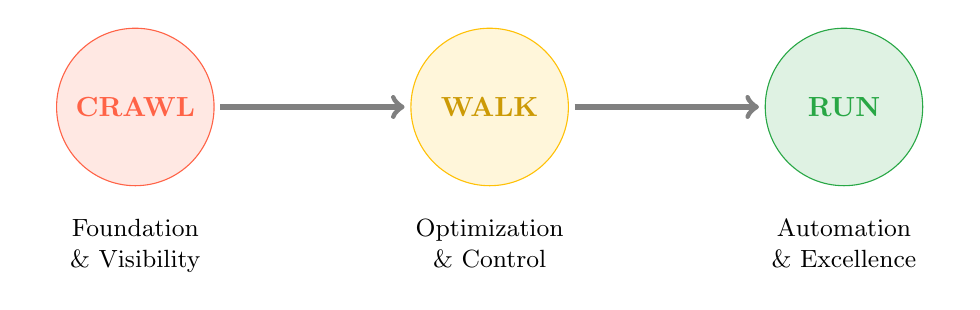
\begin{tikzpicture}[scale=0.9]
        % Crawl
        \node[circle, draw=crawlcolor, fill=crawlcolor!15, minimum size=2cm, font=\bfseries] (crawl) at (0,0) {\textcolor{crawlcolor}{CRAWL}};
        \node[below=0.3cm of crawl, font=\small, text width=2.5cm, align=center] {Foundation \& Visibility};
        
        % Walk
        \node[circle, draw=walkcolor, fill=walkcolor!15, minimum size=2cm, font=\bfseries] (walk) at (5,0) {\textcolor{walkcolor!80!black}{WALK}};
        \node[below=0.3cm of walk, font=\small, text width=2.5cm, align=center] {Optimization \& Control};
        
        % Run
        \node[circle, draw=runcolor, fill=runcolor!15, minimum size=2cm, font=\bfseries] (run) at (10,0) {\textcolor{runcolor}{RUN}};
        \node[below=0.3cm of run, font=\small, text width=2.5cm, align=center] {Automation \& Excellence};
        
        % Connecting arrows
        \draw[->, thick, gray, line width=2pt] (1.2,0) -- (3.8,0);
        \draw[->, thick, gray, line width=2pt] (6.2,0) -- (8.8,0);
    \end{tikzpicture}
    
    \vspace{2cm}
    
    {\large\textcolor{darkgray}{Roadmap Version 1.0}\\[0.3cm]}
    {\large\textcolor{darkgray}{2025 Enterprise Edition}\\[1.5cm]}
    
    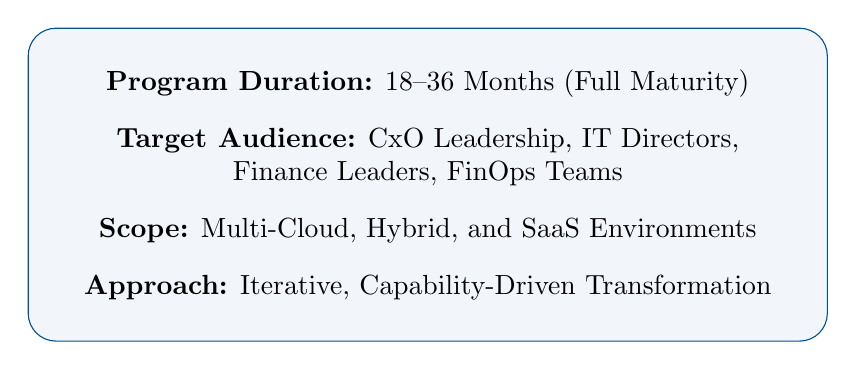
\begin{tikzpicture}
        \node[draw=primaryblue, rounded corners=10pt, inner sep=15pt, fill=primaryblue!5] {
            \begin{minipage}{0.75\textwidth}
                \centering
                \textbf{Program Duration:} 18--36 Months (Full Maturity)\\[0.3cm]
                \textbf{Target Audience:} CxO Leadership, IT Directors, Finance Leaders, FinOps Teams\\[0.3cm]
                \textbf{Scope:} Multi-Cloud, Hybrid, and SaaS Environments\\[0.3cm]
                \textbf{Approach:} Iterative, Capability-Driven Transformation
            \end{minipage}
        };
    \end{tikzpicture}
    
    \vfill
    
\end{titlepage}

% ============================================================================
% TABLE OF CONTENTS
% ============================================================================
\tableofcontents
\newpage

% ============================================================================
% CHAPTER 1: EXECUTIVE OVERVIEW
% ============================================================================
\chapter{Executive Overview}

\section{Purpose and Scope}

This Cloud FinOps Program Roadmap provides a comprehensive, technology-agnostic framework for organizations seeking to establish, mature, and sustain cloud financial management capabilities. The roadmap is designed to guide enterprises through a structured transformation journey that aligns cloud spending with business value while building sustainable organizational capabilities.

Unlike vendor-specific implementation guides, this roadmap focuses on universal principles, governance structures, and operational frameworks that apply across all cloud platforms, SaaS applications, and hybrid infrastructure environments. The methodology presented here synthesizes industry best practices, the FinOps Foundation framework, and proven enterprise transformation patterns into an actionable implementation blueprint.

\begin{keyconceptbox}
\textbf{Guiding Principle:} FinOps is not merely a cost-cutting initiative---it is a cultural and operational transformation that enables organizations to maximize the business value derived from every dollar of cloud investment while maintaining the agility and innovation velocity that cloud computing enables.
\end{keyconceptbox}

\section{Strategic Value Proposition}

Organizations that successfully implement FinOps practices realize benefits across multiple dimensions:

\subsection{Financial Benefits}

Cloud financial management maturity directly impacts the bottom line through multiple mechanisms. Cost optimization through rightsizing, commitment strategies, and waste elimination typically yields 20--35\% reduction in cloud spend within the first 12--18 months. Improved forecasting accuracy reduces budget variance from industry-average 30--40\% overruns to under 10\% deviation. Enhanced unit economics visibility enables better pricing decisions and margin management for cloud-enabled products and services.

\subsection{Operational Benefits}

Mature FinOps practices accelerate decision-making by providing real-time cost visibility to engineering teams. Automated governance reduces manual intervention while maintaining compliance. Standardized allocation methodologies eliminate monthly reconciliation disputes between business units. Proactive anomaly detection prevents bill shock and enables rapid response to cost incidents.

\subsection{Strategic Benefits}

FinOps maturity enables strategic cloud investment decisions grounded in data rather than intuition. Business units gain accountability and ownership of their technology costs, fostering responsible consumption patterns. The organization develops institutional knowledge about cloud economics that informs architecture decisions, vendor negotiations, and capacity planning.

\section{FinOps Lifecycle Overview}

The FinOps practice operates through a continuous lifecycle of three interconnected phases:

\begin{figure}[H]
\centering
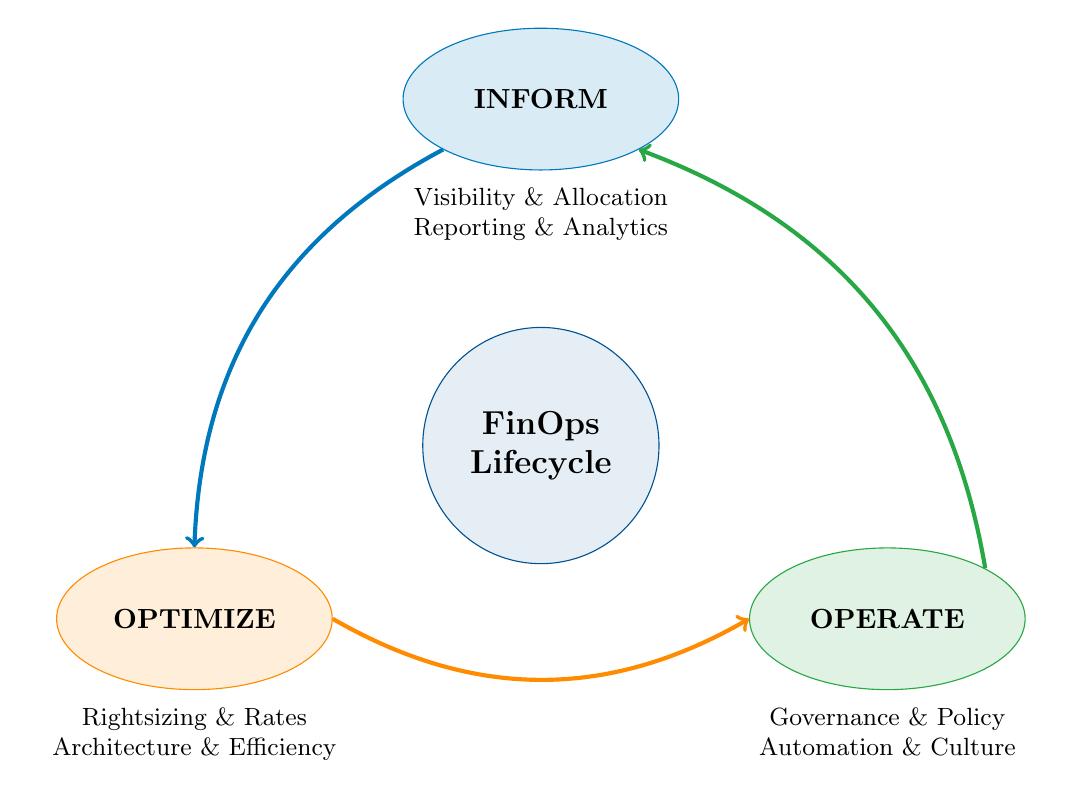
\begin{tikzpicture}[scale=1.1]
    % Central circle
    \node[circle, draw=primaryblue, fill=primaryblue!10, minimum size=3cm, font=\large\bfseries, align=center] (center) at (0,0) {FinOps\\Lifecycle};
    
    % Inform phase
    \node[ellipse, draw=secondaryblue, fill=secondaryblue!15, minimum width=3.5cm, minimum height=1.8cm, font=\bfseries] (inform) at (0,4) {INFORM};
    \node[below=0.1cm of inform.south, font=\small, text width=4cm, align=center] {Visibility \& Allocation\\Reporting \& Analytics};
    
    % Optimize phase
    \node[ellipse, draw=accentorange, fill=accentorange!15, minimum width=3.5cm, minimum height=1.8cm, font=\bfseries] (optimize) at (-4,-2) {OPTIMIZE};
    \node[below=0.1cm of optimize.south, font=\small, text width=4cm, align=center] {Rightsizing \& Rates\\Architecture \& Efficiency};
    
    % Operate phase
    \node[ellipse, draw=successgreen, fill=successgreen!15, minimum width=3.5cm, minimum height=1.8cm, font=\bfseries] (operate) at (4,-2) {OPERATE};
    \node[below=0.1cm of operate.south, font=\small, text width=4cm, align=center] {Governance \& Policy\\Automation \& Culture};
    
    % Curved arrows
    \draw[->, thick, secondaryblue, line width=1.5pt] (inform.south west) to[bend right=30] (optimize.north);
    \draw[->, thick, accentorange, line width=1.5pt] (optimize.east) to[bend right=30] (operate.west);
    \draw[->, thick, successgreen, line width=1.5pt] (operate.north east) to[bend right=30] (inform.south east);
\end{tikzpicture}
\caption{The FinOps Lifecycle: Continuous Improvement Through Inform, Optimize, Operate}
\end{figure}

\textbf{Inform Phase:} Establishing comprehensive visibility into cloud costs, usage patterns, and allocation to business units. This phase answers the questions: ``What are we spending?'' and ``Who is spending it?''

\textbf{Optimize Phase:} Taking action to improve cloud efficiency through rightsizing, rate optimization, architectural improvements, and commitment strategies. This phase answers the question: ``How can we get more value from our spend?''

\textbf{Operate Phase:} Embedding FinOps practices into organizational culture through governance, automation, and continuous improvement. This phase answers the question: ``How do we sustain and scale these practices?''

\section{Maturity Model Framework}

FinOps maturity is measured across capabilities using a three-level model that recognizes organizations progress at different rates across different capability domains:

\begin{table}[H]
\centering
\begin{tabularx}{\textwidth}{>{\bfseries}l X X X}
\toprule
\textbf{Aspect} & \textbf{Crawl} & \textbf{Walk} & \textbf{Run} \\
\midrule
Visibility & Basic cost reporting; limited allocation & Multi-dimensional analysis; accurate showback & Real-time dashboards; predictive analytics \\
\addlinespace
Optimization & Ad-hoc rightsizing; reactive adjustments & Systematic reviews; commitment strategies & Automated optimization; continuous tuning \\
\addlinespace
Governance & Manual processes; inconsistent policies & Defined standards; regular compliance checks & Policy-as-code; automated enforcement \\
\addlinespace
Culture & Centralized responsibility; low awareness & Shared accountability; growing engagement & Distributed ownership; ingrained practices \\
\addlinespace
Tooling & Native console tools; spreadsheet analysis & Integrated platform; standardized reporting & Advanced automation; ML-powered insights \\
\bottomrule
\end{tabularx}
\caption{FinOps Maturity Model Across Key Dimensions}
\end{table}

\begin{notebox}
Organizations rarely achieve uniform maturity across all capabilities simultaneously. It is common and acceptable to be at ``Run'' level for cost visibility while still at ``Crawl'' for automated optimization. The roadmap presented in subsequent chapters provides guidance for prioritizing capability development based on organizational context and strategic priorities.
\end{notebox}

\section{Roadmap Structure}

This roadmap is organized into five implementation phases that guide organizations from initial assessment through operational excellence:

\begin{figure}[H]
\centering
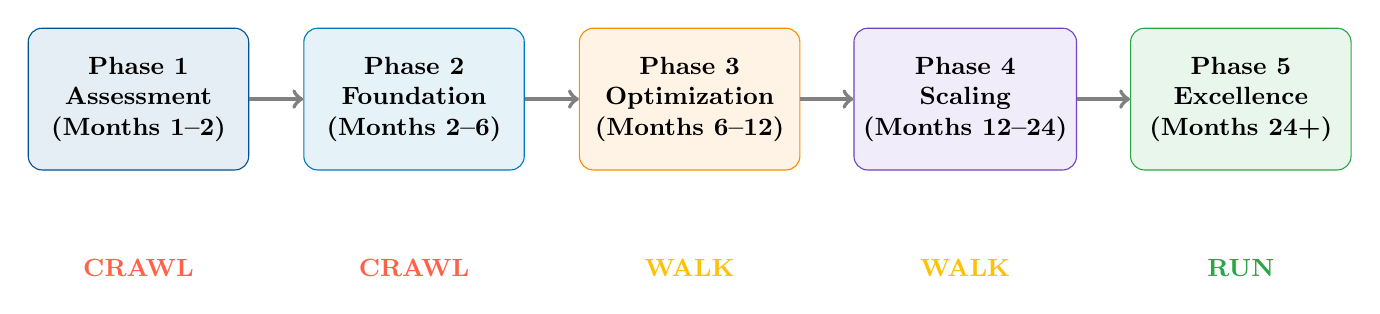
\begin{tikzpicture}[
    phase/.style={rectangle, rounded corners=5pt, draw=#1, fill=#1!10, minimum width=2.8cm, minimum height=1.8cm, align=center, font=\small\bfseries},
    arrow/.style={->, thick, gray, line width=1.5pt}
]
    \node[phase=primaryblue] (p1) at (0,0) {Phase 1\\Assessment\\(Months 1--2)};
    \node[phase=secondaryblue] (p2) at (3.5,0) {Phase 2\\Foundation\\(Months 2--6)};
    \node[phase=accentorange] (p3) at (7,0) {Phase 3\\Optimization\\(Months 6--12)};
    \node[phase=purpleaccent] (p4) at (10.5,0) {Phase 4\\Scaling\\(Months 12--24)};
    \node[phase=successgreen] (p5) at (14,0) {Phase 5\\Excellence\\(Months 24+)};
    
    \draw[arrow] (p1) -- (p2);
    \draw[arrow] (p2) -- (p3);
    \draw[arrow] (p3) -- (p4);
    \draw[arrow] (p4) -- (p5);
    
    % Maturity labels
    \node[below=1cm of p1, font=\small] {\maturitylevel{1}};
    \node[below=1cm of p2, font=\small] {\maturitylevel{1}};
    \node[below=1cm of p3, font=\small] {\maturitylevel{2}};
    \node[below=1cm of p4, font=\small] {\maturitylevel{2}};
    \node[below=1cm of p5, font=\small] {\maturitylevel{3}};
\end{tikzpicture}
\caption{Five-Phase Implementation Roadmap with Target Maturity Levels}
\end{figure}

% ============================================================================
% CHAPTER 2: ORGANIZATIONAL READINESS ASSESSMENT
% ============================================================================
\chapter{Phase 1: Organizational Readiness Assessment}

\begin{phasebox}[title=Phase 1 Overview]
\textbf{Duration:} 4--8 Weeks \hfill \textbf{Target Maturity:} Pre-Crawl to Crawl\\[0.3cm]
\textbf{Objective:} Assess current state, identify gaps, establish baseline metrics, and build the business case for FinOps investment
\end{phasebox}

\section{Current State Analysis}

Before embarking on a FinOps transformation, organizations must develop a clear understanding of their starting position. This assessment spans technical infrastructure, organizational structure, existing processes, and cultural readiness.

\subsection{Cloud Environment Discovery}

The discovery process catalogues all cloud resources, accounts, and spending across the organization. Many enterprises underestimate their cloud footprint due to shadow IT, decentralized procurement, and acquired entities with independent cloud environments.

\begin{actionbox}
\begin{enumerate}[leftmargin=*]
    \item Inventory all cloud provider accounts, subscriptions, and projects across the enterprise
    \item Document SaaS applications with significant spend (typically those exceeding \$10,000 annually)
    \item Identify hybrid infrastructure components that interact with cloud resources
    \item Map data center colocation and managed service arrangements that may migrate to cloud
    \item Catalogue cloud marketplace purchases and third-party services billed through cloud providers
\end{enumerate}
\end{actionbox}

\subsubsection{Account Structure Assessment}

Evaluate the current organization of cloud accounts and subscriptions against FinOps best practices. Key questions include:

\begin{itemize}[leftmargin=*]
    \item Are accounts organized by business unit, environment, application, or some combination?
    \item Is there a clear separation between production and non-production environments?
    \item Do account naming conventions enable easy identification of ownership and purpose?
    \item Are consolidated billing or management account structures in place?
    \item How are shared services and platform costs currently allocated?
\end{itemize}

\subsubsection{Tagging and Metadata Assessment}

Tagging is the foundation of cost allocation and accountability. Assess current tagging practices:

\begin{table}[H]
\centering
\begin{tabularx}{\textwidth}{>{\bfseries}l X c}
\toprule
\textbf{Assessment Area} & \textbf{Evaluation Criteria} & \textbf{Score (1--5)} \\
\midrule
Tag Coverage & Percentage of resources with required tags & \\
\addlinespace
Tag Accuracy & Percentage of tags with valid, current values & \\
\addlinespace
Tag Consistency & Uniformity of tag keys and value formats & \\
\addlinespace
Tag Governance & Enforcement mechanisms preventing untagged resources & \\
\addlinespace
Tag Strategy & Documented tagging standard aligned with allocation needs & \\
\bottomrule
\end{tabularx}
\caption{Tagging Maturity Assessment Scorecard}
\end{table}

\subsection{Financial Baseline Establishment}

Establishing accurate baselines is critical for measuring FinOps program success and identifying optimization opportunities.

\subsubsection{Spend Analysis}

Compile comprehensive spending data for the trailing 12 months (or as much history as available):

\begin{itemize}[leftmargin=*]
    \item Total cloud spend by provider, month, and growth trajectory
    \item Spend distribution by service category (compute, storage, network, database, analytics, etc.)
    \item Spend by business unit, cost center, or application (to the extent current tagging allows)
    \item Commitment utilization rates for existing reserved instances, savings plans, or committed use discounts
    \item Spend on cloud marketplace and third-party services
\end{itemize}

\subsubsection{Cost Efficiency Indicators}

Calculate baseline efficiency metrics that will serve as improvement targets:

\begin{table}[H]
\centering
\begin{tabularx}{\textwidth}{>{\bfseries}p{4cm} X p{3cm}}
\toprule
\textbf{Metric} & \textbf{Calculation} & \textbf{Benchmark Range} \\
\midrule
Effective Savings Rate & (On-demand equivalent -- Actual cost) / On-demand equivalent & 15--40\% \\
\addlinespace
Commitment Coverage & Committed spend / Total eligible spend & 50--80\% \\
\addlinespace
Commitment Utilization & Used committed capacity / Purchased committed capacity & 80--95\% \\
\addlinespace
Idle Resource Waste & Cost of unused resources / Total cost & $<$5\% target \\
\addlinespace
Rightsizing Opportunity & Potential savings from downsizing / Total compute cost & Varies \\
\bottomrule
\end{tabularx}
\caption{Key Efficiency Metrics and Industry Benchmarks}
\end{table}

\subsection{Organizational Structure Assessment}

FinOps success depends on organizational alignment and clear accountability structures.

\subsubsection{Stakeholder Mapping}

Identify all stakeholders who influence or are affected by cloud financial management:

\begin{table}[H]
\centering
\begin{tabularx}{\textwidth}{>{\bfseries}l X X X}
\toprule
\textbf{Stakeholder} & \textbf{Interest} & \textbf{Influence} & \textbf{Engagement Need} \\
\midrule
CFO/Finance VP & Budget accuracy, cost control & High & Executive sponsorship \\
\addlinespace
CTO/CIO & Technology strategy, innovation & High & Strategic alignment \\
\addlinespace
VP Engineering & Team velocity, developer experience & High & Operational buy-in \\
\addlinespace
Product Leaders & Unit economics, feature investment & Medium & Value understanding \\
\addlinespace
Procurement & Vendor relationships, contracts & Medium & Rate optimization \\
\addlinespace
Cloud Architects & Design patterns, standards & Medium & Technical guidance \\
\addlinespace
DevOps/Platform & Tooling, automation, operations & High & Implementation \\
\addlinespace
Business Unit Heads & P\&L ownership, budget management & High & Accountability acceptance \\
\bottomrule
\end{tabularx}
\caption{Stakeholder Mapping for FinOps Initiative}
\end{table}

\subsubsection{Current Responsibility Assessment}

Evaluate how cloud cost responsibilities are currently distributed:

\begin{itemize}[leftmargin=*]
    \item Who currently receives cloud invoices and manages payment?
    \item Who reviews cloud costs and at what frequency?
    \item Who is accountable when budgets are exceeded?
    \item Who makes commitment purchase decisions?
    \item Who has authority to implement optimization recommendations?
    \item Are there existing FinOps, cloud economics, or cost optimization roles?
\end{itemize}

\subsection{Process and Tooling Assessment}

Document existing processes and tools related to cloud financial management:

\subsubsection{Current Processes}

\begin{table}[H]
\centering
\begin{tabularx}{\textwidth}{>{\bfseries}p{4cm} X c}
\toprule
\textbf{Process Area} & \textbf{Assessment Questions} & \textbf{Exists?} \\
\midrule
Budget Planning & Is there an annual cloud budgeting process? & Yes / No / Partial \\
\addlinespace
Cost Allocation & Are costs allocated to business units monthly? & Yes / No / Partial \\
\addlinespace
Anomaly Detection & Is there monitoring for unexpected cost spikes? & Yes / No / Partial \\
\addlinespace
Optimization Reviews & Are regular rightsizing reviews conducted? & Yes / No / Partial \\
\addlinespace
Commitment Planning & Is there a strategy for reserved capacity purchases? & Yes / No / Partial \\
\addlinespace
Chargeback/Showback & Do teams see their cloud costs? & Yes / No / Partial \\
\bottomrule
\end{tabularx}
\caption{FinOps Process Maturity Assessment}
\end{table}

\subsubsection{Current Tooling}

Inventory existing tools and their capabilities:

\begin{itemize}[leftmargin=*]
    \item Cloud provider native cost management consoles and APIs
    \item Third-party cloud cost management platforms
    \item Business intelligence and visualization tools used for cost reporting
    \item Spreadsheet-based analysis and reporting
    \item Infrastructure monitoring tools with cost correlation capabilities
    \item Automation and orchestration platforms
\end{itemize}

\section{Gap Analysis and Opportunity Identification}

Compare current state findings against FinOps capability requirements to identify gaps and prioritize improvements.

\subsection{Capability Gap Assessment}

For each FinOps capability domain, assess the gap between current state and target state:

\begin{table}[H]
\centering
\small
\begin{tabularx}{\textwidth}{>{\bfseries}p{3.5cm} c c p{5.5cm}}
\toprule
\textbf{Capability} & \textbf{Current} & \textbf{Target} & \textbf{Gap Description} \\
\midrule
Cost Visibility & Crawl & Walk & Limited real-time visibility; manual reporting \\
\addlinespace
Cost Allocation & Pre-Crawl & Walk & Inconsistent tagging; no showback \\
\addlinespace
Budgeting & Crawl & Walk & Annual process only; no cloud-specific methodology \\
\addlinespace
Forecasting & Pre-Crawl & Walk & No forecasting capability \\
\addlinespace
Rate Optimization & Pre-Crawl & Crawl & No commitment strategy \\
\addlinespace
Usage Optimization & Pre-Crawl & Crawl & Occasional ad-hoc rightsizing \\
\addlinespace
Governance & Pre-Crawl & Crawl & No cost governance policies \\
\addlinespace
Organizational Alignment & Pre-Crawl & Crawl & No defined FinOps roles \\
\bottomrule
\end{tabularx}
\caption{Example Capability Gap Assessment}
\end{table}

\subsection{Quick Win Identification}

Identify optimization opportunities that can generate rapid value with minimal investment:

\begin{deliverablebox}
\textbf{Common Quick Win Categories:}
\begin{itemize}[leftmargin=*]
    \item Unused resource elimination (unattached storage, stopped instances still incurring cost, unused load balancers)
    \item Non-production environment scheduling (development and test resources running 24/7)
    \item Obvious rightsizing opportunities (significantly oversized instances with low utilization)
    \item Storage tier optimization (frequently accessed data on premium tiers, infrequent data on hot storage)
    \item Abandoned resources from previous projects or departed employees
    \item Duplicate or orphaned snapshots and backups beyond retention requirements
\end{itemize}
\end{deliverablebox}

\section{Business Case Development}

The business case for FinOps investment must quantify expected benefits, required investment, and return timeline.

\subsection{Benefit Quantification}

Estimate potential savings based on industry benchmarks adjusted for organizational context:

\begin{table}[H]
\centering
\begin{tabularx}{\textwidth}{>{\bfseries}p{4cm} c X c}
\toprule
\textbf{Optimization Category} & \textbf{Typical Savings} & \textbf{Applicability} & \textbf{Est. Value} \\
\midrule
Commitment Strategies & 20--40\% of eligible spend & Stable workloads & \$\_\_\_\_\_\_\_ \\
\addlinespace
Rightsizing & 10--30\% of compute cost & Over-provisioned resources & \$\_\_\_\_\_\_\_ \\
\addlinespace
Waste Elimination & 5--15\% of total spend & Unused resources & \$\_\_\_\_\_\_\_ \\
\addlinespace
Storage Optimization & 15--30\% of storage cost & Lifecycle management & \$\_\_\_\_\_\_\_ \\
\addlinespace
Network Optimization & 10--25\% of egress cost & Architecture improvements & \$\_\_\_\_\_\_\_ \\
\addlinespace
Architecture Improvements & Varies widely & Application modernization & \$\_\_\_\_\_\_\_ \\
\midrule
\textbf{Total Estimated Annual Savings} & & & \textbf{\$\_\_\_\_\_\_\_} \\
\bottomrule
\end{tabularx}
\caption{Savings Opportunity Sizing Template}
\end{table}

\subsection{Investment Requirements}

Calculate the investment required to build FinOps capabilities:

\begin{itemize}[leftmargin=*]
    \item \textbf{Personnel:} Dedicated FinOps team members (typically 1 FTE per \$10--20M in cloud spend)
    \item \textbf{Tooling:} Cloud cost management platform licensing (typically 1--3\% of managed spend)
    \item \textbf{Training:} Certification and skill development for FinOps and engineering teams
    \item \textbf{Consulting:} External expertise for initial implementation (optional)
    \item \textbf{Technology:} Infrastructure for automation, dashboards, and data pipelines
\end{itemize}

\subsection{ROI Calculation}

\begin{keyconceptbox}
\textbf{FinOps ROI Formula:}
\[
\text{ROI} = \frac{\text{(Annual Savings + Operational Efficiency Gains)} - \text{Program Investment}}{\text{Program Investment}} \times 100\%
\]

Industry data suggests well-implemented FinOps programs achieve 3--10x ROI within 18 months.
\end{keyconceptbox}

\section{Phase 1 Deliverables}

\begin{milestonebox}[title=Phase 1 Milestone Checklist]
\begin{itemize}[leftmargin=*]
    \item[\checkmark] Complete cloud environment inventory and account mapping
    \item[\checkmark] Establish 12-month spending baseline with trend analysis
    \item[\checkmark] Calculate current efficiency metrics (savings rate, commitment coverage, waste)
    \item[\checkmark] Complete stakeholder mapping with engagement strategy
    \item[\checkmark] Document current processes and identify gaps
    \item[\checkmark] Inventory existing tooling and assess capability gaps
    \item[\checkmark] Quantify quick win opportunities with estimated savings
    \item[\checkmark] Develop comprehensive business case with ROI projection
    \item[\checkmark] Secure executive sponsorship and budget approval
    \item[\checkmark] Define Phase 2 scope and success criteria
\end{itemize}
\end{milestonebox}

% ============================================================================
% CHAPTER 3: FOUNDATION BUILDING
% ============================================================================
\chapter{Phase 2: Foundation Building}

\begin{phasebox}[title=Phase 2 Overview]
\textbf{Duration:} 3--4 Months \hfill \textbf{Target Maturity:} Crawl\\[0.3cm]
\textbf{Objective:} Establish foundational FinOps capabilities including visibility, allocation, basic governance, and organizational structure
\end{phasebox}

\section{FinOps Team Establishment}

The FinOps function requires dedicated personnel with cross-functional skills spanning technology, finance, and organizational change management.

\subsection{Team Structure Models}

Organizations adopt different FinOps team structures based on size, culture, and cloud maturity:

\begin{table}[H]
\centering
\begin{tabularx}{\textwidth}{>{\bfseries}l c X X}
\toprule
\textbf{Model} & \textbf{Size} & \textbf{Characteristics} & \textbf{Best For} \\
\midrule
Centralized & 2--8 FTEs & Single team owns all FinOps functions & Early maturity; \$5--50M spend \\
\addlinespace
Hub-and-Spoke & 3--15 FTEs & Central team + embedded practitioners & Growing organizations; \$20--100M \\
\addlinespace
Federated & 5--25 FTEs & Distributed ownership with coordination & Large enterprises; \$100M+ spend \\
\addlinespace
Virtual/Part-Time & 0.5--2 FTEs & Shared responsibility; no dedicated team & Small cloud footprint; $<$\$5M \\
\bottomrule
\end{tabularx}
\caption{FinOps Team Structure Options}
\end{table}

\subsection{Core FinOps Roles}

Regardless of structure, several core competencies must be represented within the FinOps function:

\subsubsection{FinOps Lead/Manager}

The FinOps Lead serves as the primary driver of the FinOps practice and typically reports to IT leadership, Finance, or a dedicated Cloud Center of Excellence.

\begin{table}[H]
\centering
\begin{tabularx}{\textwidth}{>{\bfseries}l X}
\toprule
\textbf{Responsibility Area} & \textbf{Key Activities} \\
\midrule
Strategy & Define FinOps vision, roadmap, and success metrics \\
\addlinespace
Governance & Establish policies, standards, and enforcement mechanisms \\
\addlinespace
Stakeholder Management & Build relationships across engineering, finance, and business \\
\addlinespace
Reporting & Deliver executive dashboards and cost reporting \\
\addlinespace
Optimization Leadership & Drive organization-wide optimization initiatives \\
\addlinespace
Tool Administration & Oversee cost management platform and integrations \\
\bottomrule
\end{tabularx}
\caption{FinOps Lead Core Responsibilities}
\end{table}

\subsubsection{FinOps Analyst}

FinOps Analysts provide the analytical foundation for data-driven decision making.

\begin{itemize}[leftmargin=*]
    \item Develop and maintain cost allocation models and methodologies
    \item Create dashboards, reports, and visualizations for stakeholders
    \item Perform variance analysis and investigate anomalies
    \item Build forecasting models and budget projections
    \item Analyze optimization opportunities and calculate potential savings
    \item Support commitment purchase decisions with utilization analysis
\end{itemize}

\subsubsection{FinOps Engineer}

FinOps Engineers bridge the gap between financial objectives and technical implementation.

\begin{itemize}[leftmargin=*]
    \item Implement tagging strategies and automation
    \item Build data pipelines for cost and usage data
    \item Develop automation for optimization actions
    \item Create infrastructure-as-code templates with cost controls
    \item Integrate cost data with CI/CD pipelines and development workflows
    \item Implement policy-as-code for governance enforcement
\end{itemize}

\subsection{RACI Matrix for FinOps Activities}

Define clear accountability for key FinOps activities:

\begin{table}[H]
\centering
\small
\begin{tabularx}{\textwidth}{>{\raggedright\arraybackslash}p{3.5cm} c c c c c c}
\toprule
\textbf{Activity} & \textbf{FinOps} & \textbf{Eng.} & \textbf{Finance} & \textbf{Exec.} & \textbf{Procure.} & \textbf{BU} \\
\midrule
Tagging Strategy & A/R & C/I & C & I & I & I \\
Cost Allocation & A/R & C & R & I & I & C \\
Budget Setting & C & C & A/R & A & I & R \\
Rightsizing & R & A/R & I & I & I & C \\
Commitment Purchases & R & C & A & A & R & I \\
Anomaly Response & A/R & R & I & I & I & C \\
Optimization Reporting & A/R & C & C & I & I & I \\
Policy Enforcement & A/R & R & C & A & I & I \\
\bottomrule
\end{tabularx}
\caption{RACI Matrix: R=Responsible, A=Accountable, C=Consulted, I=Informed}
\end{table}

\section{Cost Visibility Infrastructure}

Visibility is the foundation of all FinOps capabilities. Without accurate, timely, and granular cost data, optimization and governance are impossible.

\subsection{Data Collection Architecture}

Design a data architecture that consolidates cost and usage data from all cloud sources:

\begin{figure}[H]
\centering
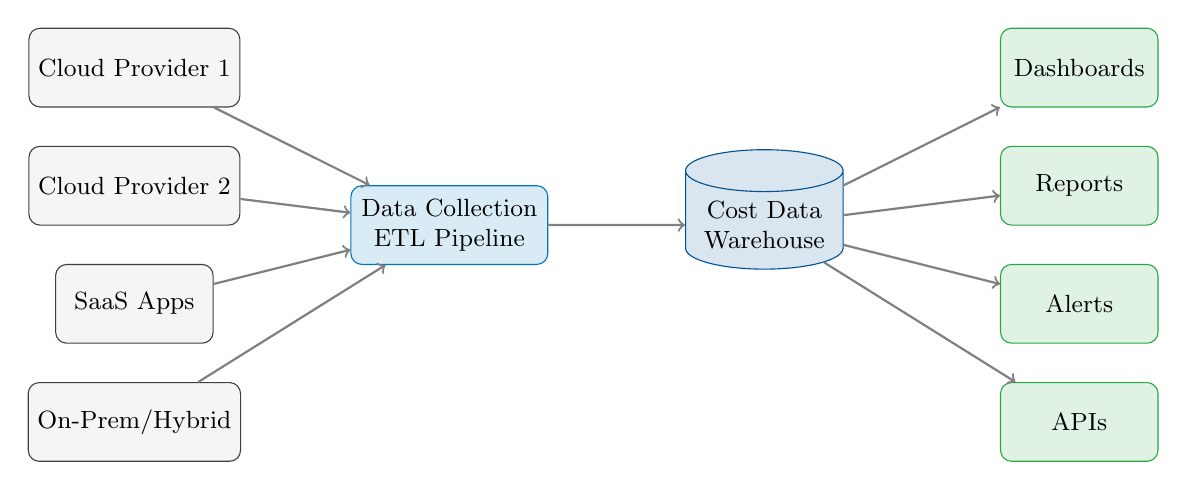
\begin{tikzpicture}[
    source/.style={rectangle, rounded corners, draw=darkgray, fill=lightgray, minimum width=2cm, minimum height=1cm, font=\small},
    process/.style={rectangle, rounded corners, draw=secondaryblue, fill=secondaryblue!15, minimum width=2.5cm, minimum height=1cm, font=\small, align=center},
    store/.style={cylinder, draw=primaryblue, fill=primaryblue!15, minimum width=2cm, minimum height=1.2cm, font=\small, shape border rotate=90, aspect=0.3, align=center},
    output/.style={rectangle, rounded corners, draw=successgreen, fill=successgreen!15, minimum width=2cm, minimum height=1cm, font=\small},
    arrow/.style={->, thick, gray}
]
    % Sources
    \node[source] (s1) at (0,4) {Cloud Provider 1};
    \node[source] (s2) at (0,2.5) {Cloud Provider 2};
    \node[source] (s3) at (0,1) {SaaS Apps};
    \node[source] (s4) at (0,-0.5) {On-Prem/Hybrid};
    
    % Collection
    \node[process] (collect) at (4,2) {Data Collection\\ETL Pipeline};
    
    % Storage
    \node[store] (store) at (8,2) {Cost Data\\Warehouse};
    
    % Outputs
    \node[output] (o1) at (12,4) {Dashboards};
    \node[output] (o2) at (12,2.5) {Reports};
    \node[output] (o3) at (12,1) {Alerts};
    \node[output] (o4) at (12,-0.5) {APIs};
    
    % Arrows
    \draw[arrow] (s1) -- (collect);
    \draw[arrow] (s2) -- (collect);
    \draw[arrow] (s3) -- (collect);
    \draw[arrow] (s4) -- (collect);
    \draw[arrow] (collect) -- (store);
    \draw[arrow] (store) -- (o1);
    \draw[arrow] (store) -- (o2);
    \draw[arrow] (store) -- (o3);
    \draw[arrow] (store) -- (o4);
\end{tikzpicture}
\caption{Cost Data Architecture Overview}
\end{figure}

\subsubsection{Data Source Integration}

For each cloud platform and service, establish data collection mechanisms:

\begin{itemize}[leftmargin=*]
    \item \textbf{Billing Data:} Detailed usage and cost records at the resource level
    \item \textbf{Usage Metrics:} Performance and utilization data for optimization analysis
    \item \textbf{Resource Metadata:} Tags, configuration, and relationship information
    \item \textbf{Commitment Inventory:} Reserved instances, savings plans, and committed use details
    \item \textbf{Pricing Data:} Rate cards, discount structures, and pricing changes
\end{itemize}

\subsubsection{Data Quality Requirements}

Establish data quality standards to ensure reliable analysis:

\begin{table}[H]
\centering
\begin{tabularx}{\textwidth}{>{\bfseries}l X c}
\toprule
\textbf{Quality Dimension} & \textbf{Requirement} & \textbf{Target} \\
\midrule
Completeness & All resources and costs captured & 100\% \\
\addlinespace
Timeliness & Data freshness for operational decisions & $<$24 hours \\
\addlinespace
Accuracy & Reconciliation with provider invoices & $>$99\% \\
\addlinespace
Granularity & Resource-level and hourly detail available & Full detail \\
\addlinespace
Consistency & Standardized formats across providers & Unified schema \\
\bottomrule
\end{tabularx}
\caption{Cost Data Quality Standards}
\end{table}

\subsection{Tagging Strategy Implementation}

Tags are the mechanism by which costs are attributed to business dimensions such as applications, teams, environments, and cost centers.

\subsubsection{Tagging Taxonomy Design}

Develop a comprehensive tagging standard that supports all allocation and reporting requirements:

\begin{table}[H]
\centering
\begin{tabularx}{\textwidth}{>{\bfseries}l l X c}
\toprule
\textbf{Tag Category} & \textbf{Example Key} & \textbf{Purpose} & \textbf{Required?} \\
\midrule
Ownership & cost-center & Financial allocation to P\&L owners & Yes \\
\addlinespace
Application & application-id & Application-level cost aggregation & Yes \\
\addlinespace
Environment & environment & Distinguish prod/non-prod; scheduling & Yes \\
\addlinespace
Project & project-code & Project-based cost tracking & Conditional \\
\addlinespace
Automation & auto-delete-after & Automated resource lifecycle & No \\
\addlinespace
Compliance & data-classification & Regulatory and security requirements & Conditional \\
\bottomrule
\end{tabularx}
\caption{Example Tagging Taxonomy}
\end{table}

\subsubsection{Tag Enforcement Mechanisms}

Implement controls to ensure tagging compliance:

\begin{actionbox}
\begin{enumerate}[leftmargin=*]
    \item Configure cloud provider policies to require tags at resource creation
    \item Implement preventive controls in infrastructure-as-code templates
    \item Deploy automated remediation to tag resources missing required tags
    \item Establish regular compliance reporting with ownership accountability
    \item Define escalation procedures for persistent non-compliance
\end{enumerate}
\end{actionbox}

\subsection{Cost Allocation Model}

Design an allocation model that distributes costs fairly and provides actionable insights to cost owners.

\subsubsection{Allocation Methodology}

\begin{table}[H]
\centering
\begin{tabularx}{\textwidth}{>{\bfseries}l X X}
\toprule
\textbf{Cost Type} & \textbf{Allocation Method} & \textbf{Considerations} \\
\midrule
Direct Costs & Tag-based attribution & Requires comprehensive tagging \\
\addlinespace
Shared Services & Proportional distribution & Based on usage, headcount, or spend \\
\addlinespace
Platform/Support & Fixed allocation or overhead & May use tiered pricing model \\
\addlinespace
Untagged Costs & Temporary holdback or default & Should be minimized over time \\
\addlinespace
Commitments & Amortization to beneficiaries & Based on actual utilization \\
\bottomrule
\end{tabularx}
\caption{Cost Allocation Methods by Cost Type}
\end{table}

\subsubsection{Showback vs. Chargeback}

Determine the appropriate model for cost accountability:

\begin{itemize}[leftmargin=*]
    \item \textbf{Showback:} Display costs to teams for awareness without P\&L impact. Appropriate for early maturity, cultural resistance, or when allocation accuracy is developing.
    \item \textbf{Chargeback:} Transfer costs to consuming business units with P\&L impact. Requires high allocation accuracy and organizational readiness.
    \item \textbf{Hybrid:} Showback for some categories, chargeback for others. Common transition approach.
\end{itemize}

\section{Basic Governance Framework}

Establish foundational governance policies and processes that create accountability without impeding agility.

\subsection{Budget Management}

Implement cloud budgeting processes that balance predictability with cloud flexibility:

\begin{itemize}[leftmargin=*]
    \item Define annual cloud budget aligned with business planning cycles
    \item Decompose budgets to business units and major cost centers
    \item Establish budget alert thresholds (e.g., 50\%, 75\%, 90\%, 100\%)
    \item Create variance review processes for budget overruns
    \item Document budget amendment procedures for justified increases
\end{itemize}

\subsection{Anomaly Detection}

Implement monitoring to detect unexpected cost changes:

\begin{warningbox}
\textbf{Anomaly Types to Monitor:}
\begin{itemize}[leftmargin=*]
    \item Day-over-day cost increases exceeding thresholds
    \item New services or regions with unexpected spend
    \item Unusual usage patterns (spikes in API calls, data transfer)
    \item Commitment expirations causing rate increases
    \item Resource proliferation in development environments
\end{itemize}
\end{warningbox}

\subsection{Policy Definition}

Document initial governance policies covering key areas:

\begin{table}[H]
\centering
\begin{tabularx}{\textwidth}{>{\bfseries}l X}
\toprule
\textbf{Policy Area} & \textbf{Example Policy Statements} \\
\midrule
Tagging & All resources must have owner, application, and environment tags \\
\addlinespace
Non-Production & Dev/test resources must be scheduled off during non-business hours \\
\addlinespace
Storage & Data older than 90 days must be moved to archival tiers \\
\addlinespace
Commitments & Reserved capacity purchases require FinOps review \\
\addlinespace
New Services & Experimental services require cost estimate before adoption \\
\bottomrule
\end{tabularx}
\caption{Example Initial Governance Policies}
\end{table}

\section{Reporting and Communication}

Establish regular reporting cadences that keep stakeholders informed and engaged.

\subsection{Executive Dashboard}

Create a monthly executive summary covering key metrics:

\begin{itemize}[leftmargin=*]
    \item Total spend and month-over-month/year-over-year trends
    \item Spend by business unit or major application
    \item Budget versus actual with variance explanations
    \item Optimization achievements and savings realized
    \item Efficiency metrics (savings rate, commitment coverage)
    \item Key initiatives status and next steps
\end{itemize}

\subsection{Team-Level Reporting}

Provide actionable reporting to engineering and product teams:

\begin{itemize}[leftmargin=*]
    \item Team/application spend trends and forecasts
    \item Optimization recommendations specific to their resources
    \item Tagging compliance status
    \item Unit cost metrics where applicable
    \item Comparison to budget and targets
\end{itemize}

\subsection{Communication Cadence}

\begin{table}[H]
\centering
\begin{tabularx}{\textwidth}{>{\bfseries}l l X l}
\toprule
\textbf{Meeting/Report} & \textbf{Frequency} & \textbf{Audience} & \textbf{Duration} \\
\midrule
Executive Review & Monthly & CFO, CTO, BU Heads & 60 min \\
\addlinespace
FinOps Working Group & Bi-weekly & Cross-functional team & 45 min \\
\addlinespace
Engineering Cost Review & Weekly & Engineering leads & 30 min \\
\addlinespace
Anomaly Triage & Daily (if needed) & FinOps + affected teams & 15 min \\
\addlinespace
Optimization Sprints & Monthly & Engineering teams & Varies \\
\bottomrule
\end{tabularx}
\caption{FinOps Communication Cadence}
\end{table}

\section{Phase 2 Deliverables}

\begin{milestonebox}[title=Phase 2 Milestone Checklist]
\begin{itemize}[leftmargin=*]
    \item[\checkmark] FinOps team established with defined roles and responsibilities
    \item[\checkmark] RACI matrix documented and communicated
    \item[\checkmark] Cost data pipeline operational with all cloud sources integrated
    \item[\checkmark] Tagging strategy documented and enforcement mechanisms active
    \item[\checkmark] Cost allocation model defined with showback/chargeback approach
    \item[\checkmark] Budget management process implemented with alerts configured
    \item[\checkmark] Anomaly detection operational with response procedures
    \item[\checkmark] Initial governance policies documented and communicated
    \item[\checkmark] Executive dashboard and team reports operational
    \item[\checkmark] Regular communication cadence established
    \item[\checkmark] Quick wins from Phase 1 implemented with savings validated
\end{itemize}
\end{milestonebox}

% ============================================================================
% CHAPTER 4: OPTIMIZATION ACCELERATION
% ============================================================================
\chapter{Phase 3: Optimization Acceleration}

\begin{phasebox}[title=Phase 3 Overview]
\textbf{Duration:} 6 Months \hfill \textbf{Target Maturity:} Walk\\[0.3cm]
\textbf{Objective:} Implement systematic optimization across all cost categories, develop commitment strategies, and establish continuous improvement processes
\end{phasebox}

\section{Rate Optimization Strategies}

Rate optimization leverages commitment mechanisms to reduce the effective cost of cloud resources.

\subsection{Commitment Portfolio Strategy}

Develop a comprehensive strategy for commitment-based discounts:

\subsubsection{Commitment Types Overview}

\begin{table}[H]
\centering
\begin{tabularx}{\textwidth}{>{\bfseries}l X c X}
\toprule
\textbf{Type} & \textbf{Characteristics} & \textbf{Discount} & \textbf{Best For} \\
\midrule
Reserved Capacity & Specific instance/resource commitment & 30--72\% & Stable, predictable workloads \\
\addlinespace
Flexible Commitments & Spend-based commitment with flexibility & 20--40\% & Variable workloads \\
\addlinespace
Spot/Preemptible & Unused capacity with interruption risk & 60--90\% & Fault-tolerant, flexible timing \\
\addlinespace
Volume Discounts & Tiered pricing based on usage volume & 5--20\% & High-volume services \\
\addlinespace
Enterprise Agreements & Negotiated enterprise contracts & Varies & Large, multi-year commitments \\
\bottomrule
\end{tabularx}
\caption{Commitment-Based Discount Mechanisms}
\end{table}

\subsubsection{Coverage and Utilization Targets}

Establish targets for commitment coverage while maintaining flexibility:

\begin{keyconceptbox}
\textbf{Commitment Planning Rule of Thumb:}
\begin{itemize}[leftmargin=*]
    \item Cover 60--70\% of stable baseline with longest-term commitments
    \item Cover additional 10--20\% with shorter-term or flexible commitments
    \item Maintain 15--25\% on-demand for burst capacity and flexibility
    \item Target 85--95\% utilization of purchased commitments
\end{itemize}
\end{keyconceptbox}

\subsubsection{Commitment Purchase Process}

Implement a governance process for commitment purchases:

\begin{enumerate}[leftmargin=*]
    \item \textbf{Analysis:} FinOps team analyzes usage patterns and identifies commitment opportunities
    \item \textbf{Recommendation:} Prepare purchase recommendation with projected savings and risks
    \item \textbf{Review:} Cross-functional review including finance and engineering stakeholders
    \item \textbf{Approval:} Obtain appropriate approval based on commitment value thresholds
    \item \textbf{Purchase:} Execute purchase through appropriate channel
    \item \textbf{Monitoring:} Track utilization and adjust strategy based on actuals
\end{enumerate}

\subsection{Spot/Preemptible Instance Strategy}

Maximize savings from interruptible compute capacity:

\begin{table}[H]
\centering
\begin{tabularx}{\textwidth}{>{\bfseries}l X X}
\toprule
\textbf{Workload Type} & \textbf{Spot Suitability} & \textbf{Implementation Approach} \\
\midrule
Batch Processing & High & Queue-based with automatic retry \\
\addlinespace
CI/CD Pipelines & High & Ephemeral build agents \\
\addlinespace
Dev/Test Environments & Medium-High & Tolerant of occasional interruption \\
\addlinespace
Containerized Workloads & Medium-High & Orchestrator handles rescheduling \\
\addlinespace
Stateless Web Tier & Medium & With robust load balancing \\
\addlinespace
Stateful Applications & Low & Requires careful architecture \\
\addlinespace
Databases/Critical & Not Recommended & Use reserved capacity instead \\
\bottomrule
\end{tabularx}
\caption{Spot Instance Suitability by Workload Type}
\end{table}

\section{Usage Optimization}

Usage optimization reduces the quantity of resources consumed through rightsizing, scheduling, and architectural improvements.

\subsection{Rightsizing Program}

Establish a systematic approach to matching resource capacity with actual requirements:

\subsubsection{Rightsizing Analysis Framework}

\begin{enumerate}[leftmargin=*]
    \item \textbf{Data Collection:} Gather utilization metrics over representative time periods (minimum 2--4 weeks)
    \item \textbf{Baseline Establishment:} Determine peak and average utilization patterns
    \item \textbf{Threshold Definition:} Set utilization targets (e.g., 70--80\% peak CPU/memory)
    \item \textbf{Opportunity Identification:} Identify resources significantly below thresholds
    \item \textbf{Recommendation Generation:} Calculate optimal size with safety margin
    \item \textbf{Validation:} Review with application owners for context
    \item \textbf{Implementation:} Execute changes through change management process
    \item \textbf{Verification:} Monitor post-change performance and costs
\end{enumerate}

\subsubsection{Rightsizing Governance}

\begin{table}[H]
\centering
\begin{tabularx}{\textwidth}{>{\bfseries}l X}
\toprule
\textbf{Governance Element} & \textbf{Implementation} \\
\midrule
Review Frequency & Monthly analysis of all compute resources \\
\addlinespace
Threshold Criteria & Resources below 40\% peak utilization flagged \\
\addlinespace
Approval Authority & Application owner approval required \\
\addlinespace
Implementation Window & Align with maintenance windows \\
\addlinespace
Rollback Plan & Quick scale-up capability if needed \\
\addlinespace
Success Metrics & Track savings realized vs. projected \\
\bottomrule
\end{tabularx}
\caption{Rightsizing Program Governance Framework}
\end{table}

\subsection{Resource Scheduling}

Implement scheduling to reduce costs for non-production environments:

\begin{actionbox}
\textbf{Scheduling Implementation Steps:}
\begin{enumerate}[leftmargin=*]
    \item Identify candidate environments (development, testing, staging, training)
    \item Define operating hours based on team locations and work patterns
    \item Implement automated start/stop mechanisms using native or third-party tools
    \item Create override procedures for after-hours access when needed
    \item Establish monitoring to verify scheduling is operating correctly
    \item Calculate and track realized savings from scheduling
\end{enumerate}
\end{actionbox}

\subsubsection{Scheduling Scenarios}

\begin{table}[H]
\centering
\begin{tabularx}{\textwidth}{>{\bfseries}l c c c}
\toprule
\textbf{Environment Type} & \textbf{Typical Schedule} & \textbf{Hours Saved/Week} & \textbf{Cost Reduction} \\
\midrule
Developer Workspaces & Weekdays 8am--6pm & 118 hours & $\sim$70\% \\
\addlinespace
QA/Test Environments & Weekdays 6am--8pm & 100 hours & $\sim$60\% \\
\addlinespace
Training Environments & As-needed basis & Varies & 80--95\% \\
\addlinespace
Demo Environments & Business hours + buffer & 80 hours & $\sim$50\% \\
\bottomrule
\end{tabularx}
\caption{Scheduling Scenarios and Expected Savings}
\end{table}

\subsection{Storage Optimization}

Optimize storage costs through lifecycle management and tiering:

\subsubsection{Storage Lifecycle Policy}

\begin{table}[H]
\centering
\begin{tabularx}{\textwidth}{c X X}
\toprule
\textbf{Age} & \textbf{Action} & \textbf{Rationale} \\
\midrule
0--30 days & Hot/Standard tier & Frequent access expected \\
\addlinespace
30--90 days & Warm/Infrequent tier & Reduced access patterns \\
\addlinespace
90--365 days & Cold/Archive tier & Rare access; compliance retention \\
\addlinespace
365+ days & Deep archive or delete & Minimal access; regulatory hold \\
\bottomrule
\end{tabularx}
\caption{Example Storage Lifecycle Policy}
\end{table}

\subsubsection{Storage Optimization Checklist}

\begin{itemize}[leftmargin=*]
    \item Implement automated lifecycle policies for object storage
    \item Review and clean up orphaned volumes and snapshots
    \item Right-size provisioned storage based on actual utilization
    \item Evaluate compression and deduplication opportunities
    \item Assess network-attached storage vs. local storage tradeoffs
    \item Review backup retention policies for cost optimization
\end{itemize}

\subsection{Network Optimization}

Reduce data transfer and network service costs:

\begin{itemize}[leftmargin=*]
    \item Analyze data transfer patterns between regions and availability zones
    \item Optimize content delivery and caching strategies
    \item Evaluate private connectivity options for high-volume transfers
    \item Review NAT gateway and load balancer utilization
    \item Implement data compression where bandwidth is costly
    \item Consider regional data residency for frequently accessed data
\end{itemize}

\section{Architectural Cost Optimization}

Address cost efficiency through architectural improvements that may require development effort.

\subsection{Containerization and Serverless}

Evaluate workloads for migration to more efficient compute models:

\begin{table}[H]
\centering
\begin{tabularx}{\textwidth}{>{\bfseries}l X X}
\toprule
\textbf{Approach} & \textbf{Cost Benefits} & \textbf{Considerations} \\
\midrule
Containerization & Higher resource utilization; efficient scaling & Orchestration complexity; learning curve \\
\addlinespace
Serverless Functions & Pay-per-execution; zero idle cost & Cold start latency; vendor lock-in \\
\addlinespace
Managed Services & Reduced operational overhead & Potential premium pricing \\
\bottomrule
\end{tabularx}
\caption{Modern Architecture Cost Considerations}
\end{table}

\subsection{Multi-Cloud and Exit Strategy}

While this roadmap is technology-agnostic, organizations should consider:

\begin{itemize}[leftmargin=*]
    \item Avoiding unnecessary lock-in through portable architectures
    \item Evaluating workload placement across providers based on pricing
    \item Maintaining negotiating leverage through credible alternatives
    \item Building abstraction layers where cost-effective
    \item Documenting exit costs and procedures for major services
\end{itemize}

\section{Forecasting and Planning}

Develop forecasting capabilities that improve budget accuracy and enable proactive planning.

\subsection{Forecasting Methodology}

\begin{table}[H]
\centering
\begin{tabularx}{\textwidth}{>{\bfseries}l X X}
\toprule
\textbf{Method} & \textbf{Approach} & \textbf{Best For} \\
\midrule
Trend-Based & Extrapolate historical patterns & Stable, organic growth \\
\addlinespace
Driver-Based & Model based on business drivers & Usage-correlated spend \\
\addlinespace
Bottom-Up & Aggregate team/project estimates & New initiatives; major changes \\
\addlinespace
Scenario Planning & Multiple scenarios with probabilities & Uncertain environments \\
\bottomrule
\end{tabularx}
\caption{Forecasting Approaches}
\end{table}

\subsection{Forecast Accuracy Improvement}

\begin{enumerate}[leftmargin=*]
    \item Track forecast versus actual monthly with variance analysis
    \item Identify systematic biases and adjust methodology
    \item Incorporate leading indicators (new projects, headcount changes, traffic trends)
    \item Build feedback loops with engineering teams for major initiatives
    \item Refine driver models based on observed correlations
\end{enumerate}

\section{Unit Economics Development}

Establish unit cost metrics that connect cloud spending to business value.

\subsection{Unit Metric Framework}

\begin{table}[H]
\centering
\begin{tabularx}{\textwidth}{>{\bfseries}l X X}
\toprule
\textbf{Business Context} & \textbf{Example Unit Metrics} & \textbf{Value} \\
\midrule
SaaS Products & Cost per user, cost per tenant & Pricing decisions; margin analysis \\
\addlinespace
E-commerce & Cost per transaction, cost per order & Profitability by channel \\
\addlinespace
Media/Content & Cost per stream, cost per impression & Content economics \\
\addlinespace
Platform Services & Cost per API call, cost per request & Usage-based pricing \\
\addlinespace
Internal IT & Cost per employee, cost per device & Benchmark comparison \\
\bottomrule
\end{tabularx}
\caption{Unit Economics Examples by Business Context}
\end{table}

\section{Phase 3 Deliverables}

\begin{milestonebox}[title=Phase 3 Milestone Checklist]
\begin{itemize}[leftmargin=*]
    \item[\checkmark] Commitment strategy documented with coverage targets
    \item[\checkmark] Initial commitment purchases executed with tracking in place
    \item[\checkmark] Spot/preemptible instance strategy implemented for eligible workloads
    \item[\checkmark] Systematic rightsizing program operational with monthly reviews
    \item[\checkmark] Non-production scheduling implemented with savings validated
    \item[\checkmark] Storage lifecycle policies deployed
    \item[\checkmark] Network optimization opportunities assessed and prioritized
    \item[\checkmark] Architectural optimization backlog established
    \item[\checkmark] Forecasting methodology implemented with accuracy tracking
    \item[\checkmark] Unit economics framework defined for key business metrics
    \item[\checkmark] Optimization savings tracking shows measurable progress
\end{itemize}
\end{milestonebox}

% ============================================================================
% CHAPTER 5: SCALING AND AUTOMATION
% ============================================================================
\chapter{Phase 4: Scaling and Automation}

\begin{phasebox}[title=Phase 4 Overview]
\textbf{Duration:} 12 Months \hfill \textbf{Target Maturity:} Walk to Run\\[0.3cm]
\textbf{Objective:} Scale FinOps practices across the enterprise, implement automation, and embed financial thinking into engineering culture
\end{phasebox}

\section{Automation Strategy}

Move from manual processes to automated workflows that scale FinOps impact without proportional team growth.

\subsection{Automation Maturity Progression}

\begin{table}[H]
\centering
\begin{tabularx}{\textwidth}{>{\bfseries}l X X}
\toprule
\textbf{Level} & \textbf{Characteristics} & \textbf{Examples} \\
\midrule
Manual & Human-driven analysis and action & Spreadsheet analysis; manual rightsizing \\
\addlinespace
Assisted & Automated insights; human action & Recommendation engines; alert systems \\
\addlinespace
Semi-Automated & Automated action with approval & Scheduled scaling with confirmation \\
\addlinespace
Fully Automated & Autonomous action within guardrails & Auto-scaling; automated scheduling \\
\bottomrule
\end{tabularx}
\caption{Automation Maturity Levels}
\end{table}

\subsection{Automation Candidates}

Prioritize automation based on impact and complexity:

\begin{table}[H]
\centering
\begin{tabularx}{\textwidth}{>{\bfseries}p{4cm} c c X}
\toprule
\textbf{Process} & \textbf{Impact} & \textbf{Complexity} & \textbf{Priority} \\
\midrule
Tagging Remediation & High & Low & \priority{1} \\
\addlinespace
Non-Prod Scheduling & High & Low & \priority{1} \\
\addlinespace
Anomaly Alerting & High & Medium & \priority{1} \\
\addlinespace
Report Generation & Medium & Low & \priority{2} \\
\addlinespace
Rightsizing Recommendations & High & Medium & \priority{2} \\
\addlinespace
Commitment Utilization Alerts & Medium & Low & \priority{2} \\
\addlinespace
Auto-Rightsizing & High & High & \priority{3} \\
\addlinespace
Dynamic Commitment Purchase & High & High & \priority{3} \\
\bottomrule
\end{tabularx}
\caption{Automation Priority Matrix}
\end{table}

\subsection{Policy-as-Code Implementation}

Implement governance policies through automated enforcement:

\begin{actionbox}
\textbf{Policy-as-Code Components:}
\begin{enumerate}[leftmargin=*]
    \item \textbf{Preventive Policies:} Block non-compliant resource creation
    \item \textbf{Detective Policies:} Identify existing non-compliant resources
    \item \textbf{Corrective Policies:} Automatically remediate violations
    \item \textbf{Reporting Policies:} Generate compliance dashboards
\end{enumerate}
\end{actionbox}

\subsection{CI/CD Integration}

Embed cost awareness into software delivery pipelines:

\begin{enumerate}[leftmargin=*]
    \item Add cost estimation to pull request reviews
    \item Include infrastructure cost impact in deployment approvals
    \item Implement cost gates for production deployments
    \item Generate cost forecasts for new feature releases
    \item Track cost trends by release or sprint
\end{enumerate}

\section{Engineering Engagement}

Scale FinOps impact by empowering engineering teams to make cost-aware decisions.

\subsection{Self-Service Capabilities}

Provide tools and dashboards that enable teams to manage their own costs:

\begin{table}[H]
\centering
\begin{tabularx}{\textwidth}{>{\bfseries}l X X}
\toprule
\textbf{Capability} & \textbf{Description} & \textbf{Benefit} \\
\midrule
Team Dashboards & Real-time cost visibility by team & Awareness and accountability \\
\addlinespace
Cost APIs & Programmatic access to cost data & Integration with team tools \\
\addlinespace
Optimization Console & Self-service rightsizing tools & Reduce FinOps bottleneck \\
\addlinespace
Budget Self-Management & Team-level budget configuration & Distributed ownership \\
\addlinespace
Anomaly Investigation & Drill-down tools for cost changes & Faster resolution \\
\bottomrule
\end{tabularx}
\caption{Self-Service FinOps Capabilities}
\end{table}

\subsection{Training and Enablement}

Build organizational capability through education:

\begin{itemize}[leftmargin=*]
    \item \textbf{FinOps Fundamentals:} Organization-wide awareness training
    \item \textbf{Role-Specific Training:} Deep dives for architects, developers, managers
    \item \textbf{Tool Training:} Hands-on workshops for cost management platforms
    \item \textbf{Certification Support:} Sponsor FinOps Foundation certifications
    \item \textbf{Lunch-and-Learns:} Regular knowledge sharing sessions
\end{itemize}

\subsection{Incentive Alignment}

Align organizational incentives with FinOps objectives:

\begin{warningbox}
\textbf{Incentive Design Considerations:}
\begin{itemize}[leftmargin=*]
    \item Balance cost efficiency with innovation velocity
    \item Avoid punitive measures that discourage cloud adoption
    \item Recognize and celebrate optimization successes
    \item Include cost awareness in engineering performance criteria
    \item Share savings benefits with teams that generate them
\end{itemize}
\end{warningbox}

\section{Multi-Cloud Governance}

Extend FinOps practices consistently across all cloud environments.

\subsection{Unified Data Model}

Normalize cost and usage data across providers:

\begin{itemize}[leftmargin=*]
    \item Develop common taxonomy for services, regions, and cost categories
    \item Standardize tagging keys and values across providers
    \item Create unified allocation methodology
    \item Establish consistent metric definitions
    \item Enable cross-provider comparison and benchmarking
\end{itemize}

\subsection{Consistent Governance}

Apply governance policies uniformly:

\begin{table}[H]
\centering
\begin{tabularx}{\textwidth}{>{\bfseries}l X}
\toprule
\textbf{Governance Area} & \textbf{Consistency Approach} \\
\midrule
Tagging Standards & Provider-agnostic tag schema with provider-specific mapping \\
\addlinespace
Budget Management & Unified budgeting process; provider-specific implementation \\
\addlinespace
Approval Workflows & Consistent thresholds; adapted to provider capabilities \\
\addlinespace
Reporting & Consolidated views with provider breakdown available \\
\addlinespace
Optimization Reviews & Unified process; provider-specific techniques \\
\bottomrule
\end{tabularx}
\caption{Multi-Cloud Governance Consistency}
\end{table}

\section{Advanced Analytics}

Leverage data and analytics for deeper insights and predictive capabilities.

\subsection{Trend Analysis}

Develop sophisticated trend analysis capabilities:

\begin{itemize}[leftmargin=*]
    \item Seasonality detection and adjustment
    \item Growth rate decomposition (organic vs. new initiatives)
    \item Cost driver correlation analysis
    \item Anomaly pattern recognition
    \item Efficiency trend monitoring
\end{itemize}

\subsection{Predictive Analytics}

Implement predictive capabilities where data supports:

\begin{itemize}[leftmargin=*]
    \item Commitment expiration impact forecasting
    \item Workload growth prediction
    \item Optimization opportunity scoring
    \item Risk assessment for commitment purchases
    \item Budget overrun early warning
\end{itemize}

\section{Vendor Management}

Leverage scale and expertise for better pricing and relationships.

\subsection{Contract Optimization}

\begin{enumerate}[leftmargin=*]
    \item Consolidate enterprise agreements where beneficial
    \item Negotiate volume discounts based on spend trajectory
    \item Establish pricing benchmarks for negotiations
    \item Review and optimize support tier selections
    \item Evaluate marketplace and reseller alternatives
\end{enumerate}

\subsection{Relationship Management}

\begin{itemize}[leftmargin=*]
    \item Establish regular business reviews with cloud providers
    \item Engage cloud provider FinOps/cost optimization teams
    \item Participate in early adopter programs for cost-relevant features
    \item Provide feedback on billing and cost management capabilities
    \item Build relationships with account teams beyond sales
\end{itemize}

\section{Phase 4 Deliverables}

\begin{milestonebox}[title=Phase 4 Milestone Checklist]
\begin{itemize}[leftmargin=*]
    \item[\checkmark] Critical automation implemented (scheduling, tagging, alerting)
    \item[\checkmark] Policy-as-code framework operational
    \item[\checkmark] CI/CD cost integration deployed
    \item[\checkmark] Self-service dashboards and tools available to teams
    \item[\checkmark] Training program established with role-specific tracks
    \item[\checkmark] Multi-cloud data normalized and unified
    \item[\checkmark] Consistent governance across cloud providers
    \item[\checkmark] Advanced analytics capabilities developed
    \item[\checkmark] Vendor management practices formalized
    \item[\checkmark] FinOps embedded in engineering culture
\end{itemize}
\end{milestonebox}

% ============================================================================
% CHAPTER 6: OPERATIONAL EXCELLENCE
% ============================================================================
\chapter{Phase 5: Operational Excellence}

\begin{phasebox}[title=Phase 5 Overview]
\textbf{Duration:} Ongoing \hfill \textbf{Target Maturity:} Run\\[0.3cm]
\textbf{Objective:} Achieve and sustain operational excellence through continuous improvement, innovation, and organizational learning
\end{phasebox}

\section{Continuous Improvement Framework}

Establish mechanisms for ongoing refinement of FinOps practices.

\subsection{Maturity Assessment Cadence}

\begin{table}[H]
\centering
\begin{tabularx}{\textwidth}{>{\bfseries}l X c}
\toprule
\textbf{Assessment Type} & \textbf{Purpose} & \textbf{Frequency} \\
\midrule
Self-Assessment & Internal capability review & Quarterly \\
\addlinespace
External Benchmark & Industry comparison & Annually \\
\addlinespace
Capability Deep-Dive & Focused improvement planning & As needed \\
\addlinespace
Stakeholder Feedback & User satisfaction and needs & Semi-annually \\
\bottomrule
\end{tabularx}
\caption{Maturity Assessment Schedule}
\end{table}

\subsection{Improvement Prioritization}

Use a structured approach to prioritize improvement initiatives:

\begin{enumerate}[leftmargin=*]
    \item \textbf{Impact Assessment:} Estimate financial and operational impact
    \item \textbf{Effort Estimation:} Evaluate implementation complexity
    \item \textbf{Risk Analysis:} Consider implementation and change risks
    \item \textbf{Strategic Alignment:} Ensure fit with organizational priorities
    \item \textbf{Sequencing:} Plan initiatives in logical order
\end{enumerate}

\section{Innovation and Emerging Practices}

Stay current with evolving FinOps practices and technologies.

\subsection{Technology Monitoring}

\begin{itemize}[leftmargin=*]
    \item Track cloud provider cost management feature releases
    \item Evaluate emerging FinOps tools and platforms
    \item Assess machine learning applications for optimization
    \item Monitor industry trends and analyst recommendations
    \item Participate in FinOps community discussions and events
\end{itemize}

\subsection{Practice Evolution}

\begin{itemize}[leftmargin=*]
    \item Incorporate sustainability and carbon considerations
    \item Extend FinOps to SaaS and software licensing
    \item Apply FinOps principles to AI/ML workloads
    \item Develop specialized practices for Kubernetes and containers
    \item Integrate with broader IT financial management
\end{itemize}

\section{Organizational Learning}

Build institutional knowledge that survives personnel changes.

\subsection{Documentation Standards}

\begin{table}[H]
\centering
\begin{tabularx}{\textwidth}{>{\bfseries}l X}
\toprule
\textbf{Document Type} & \textbf{Content} \\
\midrule
Runbooks & Step-by-step procedures for routine operations \\
\addlinespace
Decision Records & Documented rationale for key decisions \\
\addlinespace
Architecture Docs & Technical design of FinOps infrastructure \\
\addlinespace
Training Materials & Onboarding and continuing education content \\
\addlinespace
Case Studies & Success stories and lessons learned \\
\bottomrule
\end{tabularx}
\caption{FinOps Documentation Portfolio}
\end{table}

\subsection{Knowledge Sharing}

\begin{itemize}[leftmargin=*]
    \item Maintain internal wiki or knowledge base
    \item Conduct post-mortems on significant incidents
    \item Share optimization successes across teams
    \item Rotate team members through different FinOps functions
    \item Participate in external FinOps community
\end{itemize}

\section{Governance Maturation}

Evolve governance from manual enforcement to organizational habit.

\subsection{Policy Review Cycle}

\begin{enumerate}[leftmargin=*]
    \item Annual comprehensive policy review
    \item Quarterly effectiveness assessment
    \item Continuous exception tracking and analysis
    \item Regular stakeholder feedback incorporation
    \item Alignment with changing business needs
\end{enumerate}

\subsection{Compliance Excellence}

\begin{table}[H]
\centering
\begin{tabularx}{\textwidth}{>{\bfseries}l c c c}
\toprule
\textbf{Metric} & \textbf{Crawl Target} & \textbf{Walk Target} & \textbf{Run Target} \\
\midrule
Tagging Compliance & $>$70\% & $>$90\% & $>$98\% \\
\addlinespace
Budget Adherence & $\pm$30\% & $\pm$15\% & $\pm$5\% \\
\addlinespace
Policy Violations & Track & Reduce 50\% & Near zero \\
\addlinespace
Anomaly Response Time & Days & Hours & Automated \\
\bottomrule
\end{tabularx}
\caption{Governance Maturity Targets}
\end{table}

\section{Sustainability Integration}

Incorporate environmental sustainability into FinOps practices.

\subsection{Carbon-Aware Computing}

\begin{itemize}[leftmargin=*]
    \item Monitor carbon footprint of cloud usage
    \item Consider carbon intensity when selecting regions
    \item Include sustainability metrics in optimization decisions
    \item Report on environmental impact alongside financial metrics
    \item Set sustainability targets aligned with corporate goals
\end{itemize}

\subsection{Green FinOps Practices}

\begin{table}[H]
\centering
\begin{tabularx}{\textwidth}{>{\bfseries}l X}
\toprule
\textbf{Practice} & \textbf{Sustainability Impact} \\
\midrule
Rightsizing & Reduces energy consumption from unused capacity \\
\addlinespace
Scheduling & Eliminates idle resource energy waste \\
\addlinespace
Efficient Architecture & Minimizes resource requirements \\
\addlinespace
Region Selection & Can leverage lower-carbon grids \\
\addlinespace
Modern Hardware & Newer instances often more energy-efficient \\
\bottomrule
\end{tabularx}
\caption{Sustainability Benefits of FinOps Practices}
\end{table}

\section{Success Metrics and Reporting}

Demonstrate ongoing value through comprehensive metrics and reporting.

\subsection{Executive Scorecard}

\begin{table}[H]
\centering
\begin{tabularx}{\textwidth}{>{\bfseries}l X c c}
\toprule
\textbf{Metric Category} & \textbf{Key Metrics} & \textbf{Target} & \textbf{Actual} \\
\midrule
Efficiency & Effective Savings Rate & 30\%+ & \\
\addlinespace
Efficiency & Commitment Coverage & 70\%+ & \\
\addlinespace
Efficiency & Waste Rate & $<$5\% & \\
\addlinespace
Operations & Budget Variance & $\pm$10\% & \\
\addlinespace
Operations & Forecast Accuracy & 90\%+ & \\
\addlinespace
Operations & Tagging Compliance & 95\%+ & \\
\addlinespace
Value & Cost per Business Unit & Declining & \\
\addlinespace
Value & Cloud ROI & Improving & \\
\bottomrule
\end{tabularx}
\caption{Executive FinOps Scorecard Template}
\end{table}

\subsection{Value Demonstration}

\begin{itemize}[leftmargin=*]
    \item Track cumulative savings since program inception
    \item Calculate FinOps program ROI annually
    \item Document operational efficiency improvements
    \item Quantify risk reduction from governance
    \item Measure improved decision-making velocity
\end{itemize}

\section{Phase 5 Deliverables}

\begin{milestonebox}[title=Phase 5 Ongoing Objectives]
\begin{itemize}[leftmargin=*]
    \item[\checkmark] Continuous improvement framework operational
    \item[\checkmark] Regular maturity assessments conducted
    \item[\checkmark] Innovation pipeline for new capabilities
    \item[\checkmark] Comprehensive documentation maintained
    \item[\checkmark] Knowledge sharing embedded in culture
    \item[\checkmark] Governance policies regularly reviewed and updated
    \item[\checkmark] Sustainability metrics integrated into reporting
    \item[\checkmark] Executive scorecard showing consistent value
    \item[\checkmark] Industry recognition and leadership
    \item[\checkmark] FinOps practices fully embedded in organizational DNA
\end{itemize}
\end{milestonebox}

% ============================================================================
% CHAPTER 7: CHANGE MANAGEMENT
% ============================================================================
\chapter{Change Management and Cultural Transformation}

\section{The Cultural Dimension of FinOps}

FinOps is fundamentally a cultural transformation that requires changes in behavior, incentives, and organizational norms. Technical implementation without cultural change will fail to deliver sustainable results.

\subsection{Cultural Barriers}

Common cultural barriers to FinOps adoption:

\begin{table}[H]
\centering
\begin{tabularx}{\textwidth}{>{\bfseries}l X X}
\toprule
\textbf{Barrier} & \textbf{Manifestation} & \textbf{Mitigation} \\
\midrule
Engineering Resistance & ``Cost is not my job'' & Education; incentive alignment \\
\addlinespace
Fear of Constraints & Concern optimization limits innovation & Frame as value maximization \\
\addlinespace
Lack of Trust & Skepticism about data accuracy & Transparency; validation \\
\addlinespace
Accountability Avoidance & Resistance to cost ownership & Executive mandate; gradual rollout \\
\addlinespace
Short-Term Thinking & Prioritizing features over efficiency & Long-term metric tracking \\
\bottomrule
\end{tabularx}
\caption{Cultural Barriers and Mitigation Strategies}
\end{table}

\subsection{Change Management Framework}

Apply structured change management to FinOps transformation:

\begin{figure}[H]
\centering
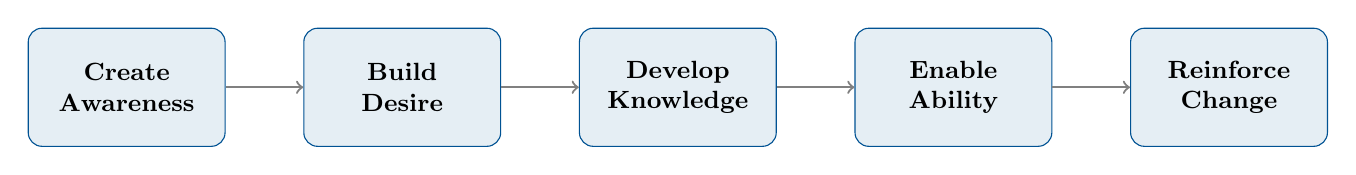
\begin{tikzpicture}[
    phase/.style={rectangle, rounded corners=5pt, draw=primaryblue, fill=primaryblue!10, minimum width=2.5cm, minimum height=1.5cm, align=center, font=\small\bfseries},
    arrow/.style={->, thick, gray}
]
    \node[phase] (aware) at (0,0) {Create\\Awareness};
    \node[phase] (desire) at (3.5,0) {Build\\Desire};
    \node[phase] (knowledge) at (7,0) {Develop\\Knowledge};
    \node[phase] (ability) at (10.5,0) {Enable\\Ability};
    \node[phase] (reinforce) at (14,0) {Reinforce\\Change};
    
    \draw[arrow] (aware) -- (desire);
    \draw[arrow] (desire) -- (knowledge);
    \draw[arrow] (knowledge) -- (ability);
    \draw[arrow] (ability) -- (reinforce);
\end{tikzpicture}
\caption{Change Management Progression (ADKAR Model)}
\end{figure}

\section{Stakeholder Engagement Strategy}

\subsection{Executive Sponsorship}

Secure and maintain active executive sponsorship:

\begin{itemize}[leftmargin=*]
    \item Identify executive champion (typically CFO, CTO, or CIO)
    \item Establish regular executive briefings
    \item Ensure visible leadership support in communications
    \item Secure executive participation in key milestones
    \item Align FinOps goals with executive performance objectives
\end{itemize}

\subsection{Engineering Engagement}

Win hearts and minds of engineering teams:

\begin{actionbox}
\textbf{Engineering Engagement Tactics:}
\begin{enumerate}[leftmargin=*]
    \item Lead with value, not cost-cutting rhetoric
    \item Provide self-service tools that reduce friction
    \item Celebrate optimization successes publicly
    \item Start with willing early adopters
    \item Address concerns directly and transparently
    \item Involve engineers in tool and process design
\end{enumerate}
\end{actionbox}

\subsection{Finance Partnership}

Build strong relationships with finance teams:

\begin{itemize}[leftmargin=*]
    \item Align cloud cost categories with financial reporting needs
    \item Establish regular collaboration on budgeting and forecasting
    \item Translate cloud metrics into financial language
    \item Support audit and compliance requirements
    \item Partner on business case development
\end{itemize}

\section{Communication Strategy}

\subsection{Communication Principles}

\begin{itemize}[leftmargin=*]
    \item \textbf{Transparency:} Share both successes and challenges openly
    \item \textbf{Relevance:} Tailor messages to audience concerns
    \item \textbf{Consistency:} Regular cadence builds trust
    \item \textbf{Two-Way:} Create channels for feedback
    \item \textbf{Celebration:} Recognize achievements prominently
\end{itemize}

\subsection{Communication Channels}

\begin{table}[H]
\centering
\begin{tabularx}{\textwidth}{>{\bfseries}l l X}
\toprule
\textbf{Channel} & \textbf{Frequency} & \textbf{Content} \\
\midrule
Executive Newsletter & Monthly & Strategic updates; key metrics \\
\addlinespace
All-Hands Update & Quarterly & Program progress; success stories \\
\addlinespace
Team Dashboards & Real-time & Operational metrics \\
\addlinespace
Slack/Teams Channel & Ongoing & Tips, alerts, discussions \\
\addlinespace
Training Sessions & As scheduled & Skill development \\
\addlinespace
Office Hours & Weekly & Q\&A; support \\
\bottomrule
\end{tabularx}
\caption{FinOps Communication Channels}
\end{table}

\section{Resistance Management}

\subsection{Identifying Resistance}

Watch for signs of resistance:

\begin{itemize}[leftmargin=*]
    \item Low engagement with dashboards and reports
    \item Persistent tagging non-compliance
    \item Skeptical questions about data accuracy
    \item Avoidance of cost discussions
    \item Complaints about ``bureaucracy''
\end{itemize}

\subsection{Addressing Resistance}

\begin{table}[H]
\centering
\begin{tabularx}{\textwidth}{>{\bfseries}l X}
\toprule
\textbf{Resistance Type} & \textbf{Response Approach} \\
\midrule
Lack of Understanding & Education; clear value articulation \\
\addlinespace
Fear of Change & Gradual rollout; quick wins first \\
\addlinespace
Competing Priorities & Executive support; integration into existing work \\
\addlinespace
Past Negative Experience & Demonstrate differences; build trust slowly \\
\addlinespace
Personal Impact Concerns & Address directly; show personal benefits \\
\bottomrule
\end{tabularx}
\caption{Resistance Response Strategies}
\end{table}

\section{Sustaining Change}

\subsection{Embedding FinOps in Operations}

Make FinOps practices part of standard operating procedures:

\begin{itemize}[leftmargin=*]
    \item Include cost reviews in sprint retrospectives
    \item Add cost considerations to architecture review boards
    \item Integrate cost metrics into deployment pipelines
    \item Include FinOps in new employee onboarding
    \item Make cost awareness part of engineering culture
\end{itemize}

\subsection{Long-Term Sustainability}

\begin{warningbox}
\textbf{Sustainability Risk Factors:}
\begin{itemize}[leftmargin=*]
    \item Executive sponsor departure
    \item FinOps team attrition
    \item Competing organizational priorities
    \item Tool or process stagnation
    \item Success leading to complacency
\end{itemize}
\end{warningbox}

% ============================================================================
% CHAPTER 8: TOOLING STRATEGY
% ============================================================================
\chapter{Tooling and Platform Strategy}

\section{Tooling Philosophy}

This roadmap deliberately avoids prescribing specific tools, recognizing that optimal tooling varies by organization size, cloud footprint, and existing technology investments. Instead, this chapter provides selection criteria and capability requirements.

\subsection{Build vs. Buy Considerations}

\begin{table}[H]
\centering
\begin{tabularx}{\textwidth}{>{\bfseries}l X X}
\toprule
\textbf{Factor} & \textbf{Favors Build} & \textbf{Favors Buy} \\
\midrule
Customization & High customization needs & Standard requirements \\
\addlinespace
Time to Value & Long runway acceptable & Rapid implementation needed \\
\addlinespace
Internal Skills & Strong data/platform team & Limited development capacity \\
\addlinespace
Integration & Deep internal system ties & Standalone acceptable \\
\addlinespace
Cost & High spend justifies investment & Lower spend; cost sensitivity \\
\addlinespace
Vendor Trust & Concerns about data sharing & Comfortable with SaaS \\
\bottomrule
\end{tabularx}
\caption{Build vs. Buy Decision Factors}
\end{table}

\section{Core Capability Requirements}

\subsection{Cost Visibility Platform}

Essential capabilities for cost visibility:

\begin{table}[H]
\centering
\begin{tabularx}{\textwidth}{>{\bfseries}l X c c c}
\toprule
\textbf{Capability} & \textbf{Description} & \textbf{Crawl} & \textbf{Walk} & \textbf{Run} \\
\midrule
Multi-Cloud Support & Ingest from all providers & Req. & Req. & Req. \\
\addlinespace
Granular Data & Resource-level, hourly detail & Nice & Req. & Req. \\
\addlinespace
Custom Allocation & Flexible cost attribution & Nice & Req. & Req. \\
\addlinespace
Historical Analysis & Multi-year trend analysis & Nice & Nice & Req. \\
\addlinespace
Real-Time Updates & Intraday data refresh & Nice & Nice & Req. \\
\addlinespace
API Access & Programmatic data retrieval & Nice & Req. & Req. \\
\bottomrule
\end{tabularx}
\caption{Cost Visibility Capability Requirements}
\end{table}

\subsection{Optimization Engine}

Capabilities for driving optimization:

\begin{itemize}[leftmargin=*]
    \item Rightsizing recommendations with utilization analysis
    \item Commitment purchase recommendations with coverage modeling
    \item Waste identification (unused, idle, orphaned resources)
    \item Storage optimization suggestions
    \item Architecture recommendations
    \item Estimated savings quantification
\end{itemize}

\subsection{Governance and Automation}

Policy and automation capabilities:

\begin{itemize}[leftmargin=*]
    \item Budget configuration and alerting
    \item Anomaly detection with configurable thresholds
    \item Policy definition and enforcement
    \item Workflow automation for common actions
    \item Integration with ticketing and notification systems
    \item Scheduled actions (start/stop, rightsizing)
\end{itemize}

\section{Evaluation Framework}

\subsection{Functional Evaluation}

\begin{table}[H]
\centering
\begin{tabularx}{\textwidth}{>{\bfseries}l X c}
\toprule
\textbf{Category} & \textbf{Evaluation Criteria} & \textbf{Weight} \\
\midrule
Data Coverage & Supported providers; data granularity & High \\
\addlinespace
Visibility & Dashboard quality; reporting flexibility & High \\
\addlinespace
Allocation & Tagging support; custom dimensions & High \\
\addlinespace
Optimization & Recommendation quality; automation & Medium \\
\addlinespace
Governance & Policy engine; workflow automation & Medium \\
\addlinespace
Integration & APIs; ecosystem connectors & Medium \\
\addlinespace
User Experience & Ease of use; learning curve & Medium \\
\bottomrule
\end{tabularx}
\caption{Platform Evaluation Criteria}
\end{table}

\subsection{Non-Functional Evaluation}

\begin{itemize}[leftmargin=*]
    \item \textbf{Security:} Data handling; compliance certifications; access controls
    \item \textbf{Scalability:} Ability to handle growth in data volume and users
    \item \textbf{Performance:} Query response times; dashboard load times
    \item \textbf{Reliability:} Uptime guarantees; data accuracy
    \item \textbf{Support:} Implementation assistance; ongoing support quality
    \item \textbf{Roadmap:} Vendor investment; feature development trajectory
\end{itemize}

\subsection{Commercial Evaluation}

\begin{itemize}[leftmargin=*]
    \item Pricing model (percentage of managed spend, flat fee, per-user)
    \item Total cost of ownership including implementation and training
    \item Contract flexibility (term, scaling, exit provisions)
    \item Proof-of-concept or trial availability
    \item Reference customer availability
\end{itemize}

\section{Implementation Approach}

\subsection{Phased Rollout}

\begin{enumerate}[leftmargin=*]
    \item \textbf{Pilot:} Implement with limited scope; validate capabilities
    \item \textbf{Expand:} Extend to additional teams and cloud accounts
    \item \textbf{Integrate:} Connect with organizational systems
    \item \textbf{Automate:} Enable advanced automation features
    \item \textbf{Optimize:} Tune and customize for organizational needs
\end{enumerate}

\subsection{Success Criteria}

Define measurable success criteria for platform implementation:

\begin{itemize}[leftmargin=*]
    \item Time to first actionable insight
    \item User adoption rate (active users / licensed users)
    \item Data accuracy (reconciliation with invoices)
    \item Optimization savings attributable to platform
    \item Stakeholder satisfaction scores
\end{itemize}

% ============================================================================
% CHAPTER 9: RISK MANAGEMENT
% ============================================================================
\chapter{Risk Management}

\section{Program Risk Categories}

\subsection{Implementation Risks}

\begin{table}[H]
\centering
\begin{tabularx}{\textwidth}{>{\bfseries}p{3cm} X X c}
\toprule
\textbf{Risk} & \textbf{Description} & \textbf{Mitigation} & \textbf{Level} \\
\midrule
Data Quality & Incomplete or inaccurate cost data & Validation processes; reconciliation & High \\
\addlinespace
Adoption & Low stakeholder engagement & Change management; incentives & High \\
\addlinespace
Resource Constraints & Insufficient team capacity & Phased approach; automation & Medium \\
\addlinespace
Technical Complexity & Integration challenges & Proof-of-concepts; expertise & Medium \\
\addlinespace
Tool Selection & Poor platform fit & Thorough evaluation; pilots & Medium \\
\bottomrule
\end{tabularx}
\caption{Implementation Risk Assessment}
\end{table}

\subsection{Operational Risks}

\begin{table}[H]
\centering
\begin{tabularx}{\textwidth}{>{\bfseries}p{3cm} X X c}
\toprule
\textbf{Risk} & \textbf{Description} & \textbf{Mitigation} & \textbf{Level} \\
\midrule
Over-Optimization & Performance impact from aggressive rightsizing & Testing; guardrails; rollback & High \\
\addlinespace
Commitment Lock-In & Stranded reserved capacity & Conservative coverage; flexibility & Medium \\
\addlinespace
Knowledge Concentration & Dependence on key individuals & Documentation; cross-training & Medium \\
\addlinespace
Alert Fatigue & Overwhelming notifications & Threshold tuning; prioritization & Low \\
\bottomrule
\end{tabularx}
\caption{Operational Risk Assessment}
\end{table}

\subsection{Organizational Risks}

\begin{table}[H]
\centering
\begin{tabularx}{\textwidth}{>{\bfseries}p{3cm} X X c}
\toprule
\textbf{Risk} & \textbf{Description} & \textbf{Mitigation} & \textbf{Level} \\
\midrule
Sponsor Loss & Executive champion leaves & Multiple sponsors; institutionalize & High \\
\addlinespace
Priority Shift & Competing organizational priorities & Demonstrate value; maintain visibility & Medium \\
\addlinespace
Culture Clash & Resistance to accountability & Gradual change; positive framing & Medium \\
\addlinespace
Skill Gaps & Inability to hire/develop talent & Training; managed services & Medium \\
\bottomrule
\end{tabularx}
\caption{Organizational Risk Assessment}
\end{table}

\section{Risk Monitoring}

Establish ongoing risk monitoring processes:

\begin{itemize}[leftmargin=*]
    \item Quarterly risk assessment reviews
    \item Key risk indicators tracked on dashboards
    \item Escalation procedures for emerging risks
    \item Regular stakeholder feedback collection
    \item Post-incident reviews for realized risks
\end{itemize}

% ============================================================================
% CHAPTER 10: APPENDICES
% ============================================================================
\appendix

\chapter{Assessment Templates}

\section{Organizational Readiness Scorecard}

\begin{table}[H]
\centering
\small
\begin{tabularx}{\textwidth}{X c c c c c}
\toprule
\textbf{Readiness Dimension} & \textbf{1} & \textbf{2} & \textbf{3} & \textbf{4} & \textbf{5} \\
\midrule
Executive support for FinOps initiative & $\circ$ & $\circ$ & $\circ$ & $\circ$ & $\circ$ \\
\addlinespace
Cross-functional collaboration culture & $\circ$ & $\circ$ & $\circ$ & $\circ$ & $\circ$ \\
\addlinespace
Data-driven decision making maturity & $\circ$ & $\circ$ & $\circ$ & $\circ$ & $\circ$ \\
\addlinespace
Current cost visibility capabilities & $\circ$ & $\circ$ & $\circ$ & $\circ$ & $\circ$ \\
\addlinespace
Engineering engagement with costs & $\circ$ & $\circ$ & $\circ$ & $\circ$ & $\circ$ \\
\addlinespace
Finance cloud cost understanding & $\circ$ & $\circ$ & $\circ$ & $\circ$ & $\circ$ \\
\addlinespace
Change management capabilities & $\circ$ & $\circ$ & $\circ$ & $\circ$ & $\circ$ \\
\addlinespace
Available funding for initiative & $\circ$ & $\circ$ & $\circ$ & $\circ$ & $\circ$ \\
\midrule
\textbf{Total Score} & \multicolumn{5}{c}{\_\_\_\_ / 40} \\
\bottomrule
\end{tabularx}
\caption{Organizational Readiness Assessment (1=Low, 5=High)}
\end{table}

\section{Capability Maturity Assessment}

\begin{table}[H]
\centering
\small
\begin{tabularx}{\textwidth}{X c c c c}
\toprule
\textbf{Capability} & \textbf{None} & \textbf{Crawl} & \textbf{Walk} & \textbf{Run} \\
\midrule
Cost Visibility \& Reporting & $\circ$ & $\circ$ & $\circ$ & $\circ$ \\
\addlinespace
Cost Allocation \& Tagging & $\circ$ & $\circ$ & $\circ$ & $\circ$ \\
\addlinespace
Budgeting \& Forecasting & $\circ$ & $\circ$ & $\circ$ & $\circ$ \\
\addlinespace
Anomaly Detection & $\circ$ & $\circ$ & $\circ$ & $\circ$ \\
\addlinespace
Rate Optimization & $\circ$ & $\circ$ & $\circ$ & $\circ$ \\
\addlinespace
Usage Optimization & $\circ$ & $\circ$ & $\circ$ & $\circ$ \\
\addlinespace
Governance \& Policies & $\circ$ & $\circ$ & $\circ$ & $\circ$ \\
\addlinespace
Automation & $\circ$ & $\circ$ & $\circ$ & $\circ$ \\
\addlinespace
Organizational Alignment & $\circ$ & $\circ$ & $\circ$ & $\circ$ \\
\addlinespace
Cultural Adoption & $\circ$ & $\circ$ & $\circ$ & $\circ$ \\
\bottomrule
\end{tabularx}
\caption{Capability Maturity Assessment}
\end{table}

\chapter{Key Performance Indicators}

\section{Efficiency Metrics}

\begin{table}[H]
\centering
\begin{tabularx}{\textwidth}{>{\bfseries}l X}
\toprule
\textbf{Metric} & \textbf{Formula} \\
\midrule
Effective Savings Rate & (On-Demand Equivalent -- Actual Cost) / On-Demand Equivalent \\
\addlinespace
Commitment Coverage & Committed Spend / Total Eligible Spend \\
\addlinespace
Commitment Utilization & Used Committed Capacity / Purchased Capacity \\
\addlinespace
Waste Rate & Unused Resource Cost / Total Cost \\
\addlinespace
Rightsizing Opportunity & Potential Savings from Rightsizing / Total Compute Cost \\
\bottomrule
\end{tabularx}
\caption{Efficiency Metric Definitions}
\end{table}

\section{Operational Metrics}

\begin{table}[H]
\centering
\begin{tabularx}{\textwidth}{>{\bfseries}l X}
\toprule
\textbf{Metric} & \textbf{Formula} \\
\midrule
Tagging Compliance & Tagged Resources / Total Resources \\
\addlinespace
Budget Variance & |Forecast -- Actual| / Actual \\
\addlinespace
Forecast Accuracy & 1 -- (|Forecast -- Actual| / Actual) \\
\addlinespace
Anomaly Detection Rate & Detected Anomalies / Total Anomalies \\
\addlinespace
Mean Time to Optimization & Average Time from Identification to Remediation \\
\bottomrule
\end{tabularx}
\caption{Operational Metric Definitions}
\end{table}

\section{Business Value Metrics}

\begin{table}[H]
\centering
\begin{tabularx}{\textwidth}{>{\bfseries}l X}
\toprule
\textbf{Metric} & \textbf{Formula} \\
\midrule
Cost per Business Unit & Cloud Cost / Business Unit (Transaction, User, Revenue) \\
\addlinespace
Cloud ROI & (Business Value -- Cloud Cost) / Cloud Cost \\
\addlinespace
FinOps Program ROI & (Savings Realized -- Program Cost) / Program Cost \\
\addlinespace
Cumulative Savings & Sum of All Verified Savings Since Program Start \\
\bottomrule
\end{tabularx}
\caption{Business Value Metric Definitions}
\end{table}

\chapter{Glossary of Terms}

\begin{description}[leftmargin=!,labelwidth=4.5cm]
    \item[Allocation] The process of attributing cloud costs to cost centers, applications, or teams
    \item[Amortization] Spreading commitment costs over the commitment term
    \item[Anomaly] An unexpected deviation from normal cost patterns
    \item[Chargeback] Transferring cloud costs to consuming business units with P\&L impact
    \item[Commitment] Pre-purchased capacity or spend for discounted rates
    \item[Coverage] The percentage of eligible usage covered by commitments
    \item[FinOps] Cloud Financial Operations---the practice of managing cloud costs
    \item[Forecast] Prediction of future cloud spending
    \item[Maturity Model] Framework for assessing FinOps capability development
    \item[On-Demand] Cloud resources consumed without commitments at list price
    \item[Optimization] Actions taken to improve cloud cost efficiency
    \item[Reserved Capacity] Pre-purchased specific resource capacity
    \item[Rightsizing] Adjusting resource size to match actual utilization
    \item[Savings Plan] Flexible commitment for compute usage
    \item[Showback] Displaying costs to teams without P\&L impact
    \item[Spot Instance] Unused capacity at steep discount with interruption risk
    \item[Tagging] Metadata attached to resources for cost allocation
    \item[Unit Economics] Cost metrics normalized by business units
    \item[Utilization] The percentage of purchased commitment actually used
    \item[Waste] Costs incurred for resources that provide no value
\end{description}

\chapter{Implementation Checklist}

\section{Phase 1 Checklist: Assessment}

\begin{itemize}[leftmargin=*]
    \item[$\square$] Complete cloud environment inventory
    \item[$\square$] Establish 12-month spending baseline
    \item[$\square$] Calculate current efficiency metrics
    \item[$\square$] Complete stakeholder mapping
    \item[$\square$] Document current processes
    \item[$\square$] Assess current tooling
    \item[$\square$] Identify quick win opportunities
    \item[$\square$] Develop business case
    \item[$\square$] Secure executive sponsorship
    \item[$\square$] Obtain budget approval
\end{itemize}

\section{Phase 2 Checklist: Foundation}

\begin{itemize}[leftmargin=*]
    \item[$\square$] Establish FinOps team
    \item[$\square$] Define roles and RACI
    \item[$\square$] Implement cost data pipeline
    \item[$\square$] Deploy tagging strategy
    \item[$\square$] Establish cost allocation model
    \item[$\square$] Implement budget management
    \item[$\square$] Configure anomaly detection
    \item[$\square$] Document initial policies
    \item[$\square$] Create executive dashboard
    \item[$\square$] Establish communication cadence
\end{itemize}

\section{Phase 3 Checklist: Optimization}

\begin{itemize}[leftmargin=*]
    \item[$\square$] Develop commitment strategy
    \item[$\square$] Execute initial commitments
    \item[$\square$] Implement spot/preemptible strategy
    \item[$\square$] Establish rightsizing program
    \item[$\square$] Deploy non-production scheduling
    \item[$\square$] Implement storage lifecycle policies
    \item[$\square$] Assess network optimization
    \item[$\square$] Create architecture backlog
    \item[$\square$] Implement forecasting
    \item[$\square$] Define unit economics
\end{itemize}

\section{Phase 4 Checklist: Scaling}

\begin{itemize}[leftmargin=*]
    \item[$\square$] Implement critical automation
    \item[$\square$] Deploy policy-as-code
    \item[$\square$] Integrate with CI/CD
    \item[$\square$] Provide self-service tools
    \item[$\square$] Establish training program
    \item[$\square$] Normalize multi-cloud data
    \item[$\square$] Ensure consistent governance
    \item[$\square$] Develop advanced analytics
    \item[$\square$] Formalize vendor management
    \item[$\square$] Embed in engineering culture
\end{itemize}

\section{Phase 5 Checklist: Excellence}

\begin{itemize}[leftmargin=*]
    \item[$\square$] Establish continuous improvement
    \item[$\square$] Conduct regular assessments
    \item[$\square$] Maintain innovation pipeline
    \item[$\square$] Keep documentation current
    \item[$\square$] Foster knowledge sharing
    \item[$\square$] Review policies regularly
    \item[$\square$] Integrate sustainability
    \item[$\square$] Report executive metrics
    \item[$\square$] Pursue industry recognition
    \item[$\square$] Sustain organizational embedding
\end{itemize}

% ============================================================================
% END MATTER
% ============================================================================

\chapter*{About This Roadmap}
\addcontentsline{toc}{chapter}{About This Roadmap}

This Cloud FinOps Program Roadmap synthesizes industry best practices, the FinOps Foundation framework, and proven enterprise transformation methodologies into a comprehensive, technology-agnostic implementation guide.

The roadmap is designed to be adapted to organizational context. Not every element will apply to every organization, and implementation timelines should be adjusted based on organizational size, cloud footprint, and strategic priorities.

\vspace{1cm}

\begin{notebox}
\textbf{Continuous Improvement:} This roadmap should be treated as a living document, updated regularly to reflect evolving FinOps practices, organizational learning, and changing cloud economics.
\end{notebox}

\vfill

\begin{center}
\textit{Cloud FinOps Program Roadmap}\\
\textit{Version 1.0 --- 2025 Enterprise Edition}
\end{center}

\end{document}